%% Setup
\documentclass[10pt,a4paper]{article}
\usepackage{amsmath,amssymb,amsfonts,graphicx,geometry,booktabs,xcolor,setspace,hyperref,siunitx,listings,float,enumitem,titlesec,subcaption,authblk,placeins,sectsty,fancyhdr}
\usepackage[capitalise]{cleveref}
\usepackage[labelfont=bf]{caption} % Bold figure/table titles
\hypersetup{hidelinks}
\usepackage[style=authoryear,natbib=true]{biblatex}
\addbibresource{literature.bib}
\setstretch{1.15}
\hypersetup{
    colorlinks=true,
    linkcolor=blue!70!black,
    urlcolor=blue!70!black,
    citecolor=blue!70!black,
}
\definecolor{mitred}{rgb}{0.639,0.122,0.204}
\lstset{
    basicstyle=\ttfamily\small,
    keywordstyle=\color{blue},
    commentstyle=\color{gray},
    stringstyle=\color{orange!80!black},
    frame=single,
    breaklines=true,
    numbers=left,
    numberstyle=\tiny\color{gray},
    language=Python,
}
\geometry{margin=2.5cm,bottom=3cm,footskip=40pt}
\pagestyle{fancy}
\fancyhead[R]{MIT\ 16.122}
\fancyfoot[L]{\raisebox{-0.5\baselineskip}{
\includegraphics[width=3cm]{figures/mit-lockup-red.png}}}
\fancyfoot[R]{\sffamily\textbf{\thepage}}
\fancyfoot[C]{}

%% Metadata
\title{\sffamily\textbf{\normalsize MIT 16.122 --- Hypersonic Aerothermodynamics}\\ Preliminary Design of a Hypersonic Passenger Aircraft}
\date{\sffamily\today}
\author[1,3,4]{Zachary Durocher}
\author[1,3,4]{Andrew Nguyen}
\author[1,2]{Th\'eo Rulko}
\affil[1]{Department of Aeronautics \& Astronautics, Massachusetts Institute of Technology}
\affil[2]{MIT-NNSA Center for the Exascale Simulation of High-Enthalpy Fluid-Solid Interactions (CHEFSI)}
\affil[3]{MIT Hypersonics Research Laboratory (HRL)}
\affil[4]{United States Air Force}
\usepackage{amsmath}
\renewcommand\Affilfont{\itshape\small}
\setlength\parindent{0pt}
\graphicspath{{../runs/}}

% ==========================================================================
\begin{document}
\allsectionsfont{\sffamily}
\maketitle%

% ==========================================================================
\section*{\large Executive Summary}
Using a cone-derived waverider geometry, a hypersonic 100-passenger aircraft is designed to cruise from Sweden to Singapore in approximately 2.5~hours, traveling at Mach~6 at an altitude of 70,000~ft. The external vehicle geometry is parameterized and optimized for minimum drag, thereby minimizing the required thrust and, ultimately, the size of the aircraft. Key sizing outcomes for the final design are presented in Table \ref{tab:breguet_optimizer_best_case}. 
\\\\
The design process follows Bowcutt's \citep{Bowcutt:1986,Bowcutt:1987} viscous-optimized waverider paper. An algorithm is implemented, taking freestream conditions and vehicle geometry parameters as inputs, then calculating surface pressure, shear, and temperature values as well as vehicle performance metrics as outputs. A constrained optimization is run to find a waverider geometry which minimizes thrust required, subject to payload size constraints.
\\\\
In modeling the flow physics, a steady laminar continuum flow is assumed, and separation is not modeled, so the wake at the flat base of the vehicle is not considered. The Taylor-Maccol inviscid flow around a cone is utilized in generating waverider geometries. Walz's compressible laminar boundary layer method with an isothermal wall is then used in predicting viscous drag on the waverider. Aerothermal heating assuming radiative equilibrium is considered for the purpose of predicting the radius of a real blunt leading edge, and the blunt pressure drag contribution is calculated using modified Newtonian theory. Along the chosen flight path, geographically varying freestream properties are accounted for using NRLMSISE models.
\\\\
After defining an optimized exterior geometry, selection and optimization of additional design parameters is performed. Thermal protection system material is chosen based on leading edge temperature requirements. Engine sizing and fuel quantity are determined using the Breguet range equation and a fixed engine thrust-to-weight ratio assumption. While some key subsystems and performance elements (namely, those related to takeoff and landing) are not accounted for, the design and analysis presented below offers a reasonable, physically-based foundation upon which future work can build.

\begin{table}[H]
\centering
\caption{Summary of the characteristics of the proposed vehicle}
\begin{tabular}{l r l}
\hline
\textbf{Parameter} & \textbf{Value} & \textbf{Units} \\
\hline

Takeoff mass & 51,220 & kg \\
Takeoff weight & 502,000 & N \\

Required fuel mass & 23,550 & kg \\
Required fuel volume & 29.3 & m$^3$ \\
Fuel volume fraction & 12 & \% \\
Fuel & JP-7 & -- \\

Length & 29.8 & m \\
Wingspan & 15.6 & m \\
Total internal volume & 250 & m$^2$ \\
Cabin height & 3.08 & m \\

Specific impulse & 2,500 & s \\
Engine count & 6 & -- \\
Available thrust & 360,000 & N \\
Required thrust with margin & 245,000 & N \\
Powerplant mass & 2,500 & kg \\
Mass per engine & 417 & kg \\

Maximum skin temperature & 2500 & K \\
Maximum skin shear stress & 8.14 & kPa \\



\hline
\end{tabular}
\label{tab:breguet_optimizer_best_case}
\end{table}
\tableofcontents%
\setlength{\parskip}{1ex}%

%% Body
\section{Introduction}
\label{sec:intro}
The goal of this project is to develop a commercial hypersonic vehicle capable of carrying passengers over the Arctic Circle between Uppsala, Sweden and Singapore. This report presents a preliminary design for such a vehicle, detailing initial aerodynamic shape, size, and weight estimates, propulsion characteristics, and material selection, and outlining the methodology used to justify design decisions.



% ==========================================================================
\section{Concept of Mission Operations (ConOps)}\label{sec:conops}
\subsection{Design constraints}\label{sec:constraints}
The proposed design must satisfy the following constraints:
\begin{enumerate}[label=\roman*.,noitemsep]
    \item The vehicle must fly over the Arctic Circle from Uppsala, Sweden, to Singapore;
    \item The vehicle must carry a minimum of 100 passengers;
    \item The vehicle must fly at a cruising altitude between 50,000 and 70,000 ft;
    \item The vehicle must fly at a cruising speed between Mach 4 and Mach 6; and
    \item In addition to the specified points of departure and arrival, the route taken by the vehicle must also fly over the Gulf of Bothnia, Greenland, the Arctic Ocean, the Pacific Ocean, and the South China Sea.
\end{enumerate}

To minimize flight time, while also operating at the altitude where the freestream density is lowest within the allowable envelope (and thus where aerodynamic drag and aerothermal heat flux are smallest), the team selected Mach~6 flight at a cruising altitude of 70,000~ft. This choice of Mach number enables the use of scramjets, whose efficient operation requires a high supersonic inlet flow (typically $M_\infty \gtrsim 5$) and which become the only practical airbreathing option in this regime (see~\cref{sec:propulsion}). Per the design brief, maneuvering, takeoff, and landing are neglected, and the vehicle is optimized for steady, level flight.

\subsection{Flight path selection}\label{sec:trajectory}

To determine the minimum-distance route from Uppsala to Singapore while flying over the Gulf of Bothnia, Greenland, the Arctic Ocean, the Pacific Ocean, and the South China Sea, flight path selection was formulated as a constrained optimization problem in spherical coordinates.

The departure point (Uppsala) and destination (Singapore) were treated as fixed geographic coordinates. The intermediate locations were not imposed as exact waypoints; instead, each was modeled as a circular flyover region centered on a representative latitude and longitude with an assigned radius. This reflects the requirement that the vehicle only needs to pass over each area of interest, rather than intersect at an exact point.

\begin{figure}[htb!]
    \centering
    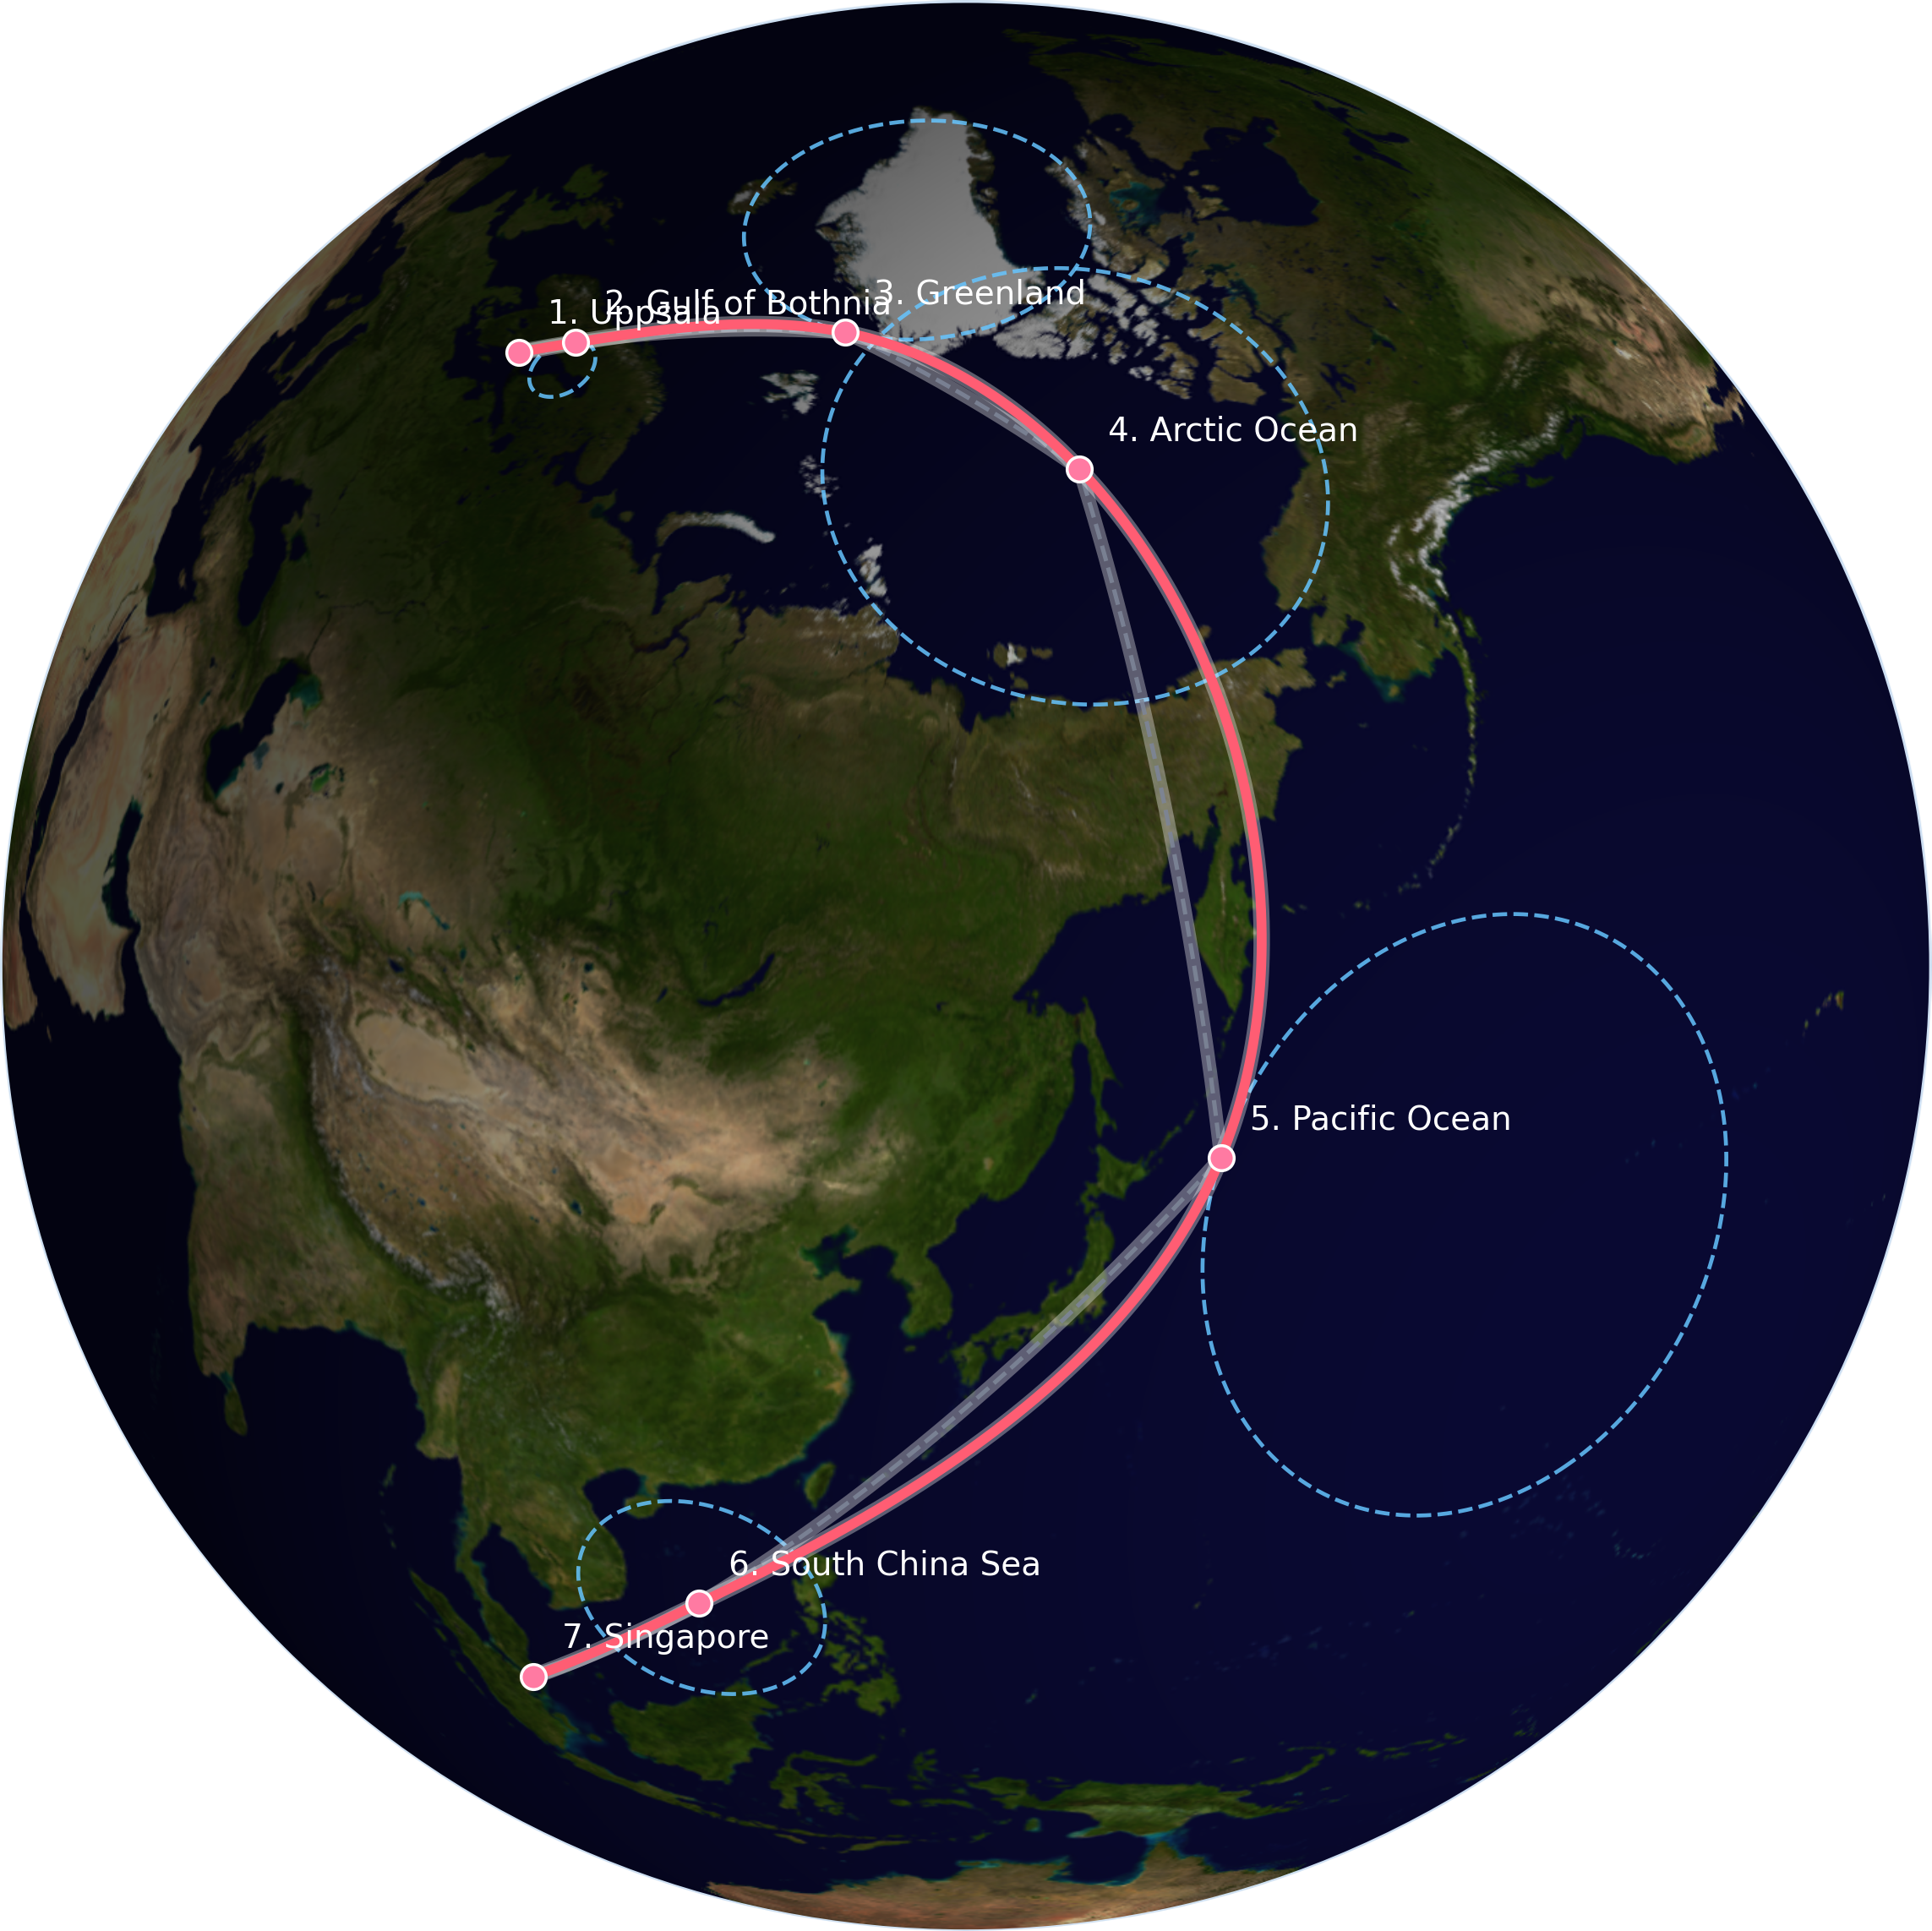
\includegraphics[width=0.6\linewidth]{route_visualization/plots/route_orthographic.png}
    \caption{Optimized Route. The dotted circle regions denote the `radius' of points of interest.}
    \label{fig:route}
\end{figure}

% \begin{figure}[htb!]
%     \centering
%     
\includegraphics[width=1\linewidth]{Route Visualized 2D Projection.png}
%     \caption{2D Projection of the selected route}
%     \label{fig:placeholder}
% \end{figure}

For any two points on the surface of the Earth, the separation was computed as a great-circle arc. If the two points have latitude-longitude coordinates $(\phi_1,\lambda_1)$ and $(\phi_2,\lambda_2)$, the central angle between them is
\begin{equation}
    \Delta \sigma =\cos^{-1}\left(\sin\phi_1 \sin\phi_2+\cos\phi_1 \cos\phi_2 \cos(\lambda_2-\lambda_1)\right).
\end{equation}
The corresponding surface distance is then
\begin{equation}
    s = R_E \Delta \sigma,
\end{equation}
where $R_E$ is the Earth radius.

Each flyover point inside a region was parameterized by two variables: a bearing angle and a fractional radius. A numerical optimizer was then used to vary the bearing and radial position of each intermediate crossing point to minimize the total route length. Starting from the region center, a candidate crossing point was generated by moving outward along a specified bearing by a distance between $0$ and the full region radius. This allowed the optimizer to place the actual crossing point anywhere inside the flyover region. Multiple initial guesses were provided to reduce sensitivity to local minima, and the best-converged solution was retained. 

Once the minimum-distance sequence of anchor points was found, a smooth spine curve was generated so that the route would not contain sharp corners. The optimized latitude--longitude anchor points were first converted to 3D Cartesian coordinates on the unit sphere. A cubic spline was then fit separately to the $x$, $y$, and $z$ coordinates as functions of cumulative path distance. The spline was sampled densely, and each sample point was renormalized to the sphere. This produced a smooth route that passes through the optimized anchor points while remaining on the Earth-centered spherical surface. The flight path is shown on~\cref{fig:route}.

Finally, the route distance was evaluated for a constant cruise altitude of $70{,}000$~ft. Since this corresponds to motion on a sphere of radius $R_E+h$, where $h=70{,}000$~ft, the flight-path distance for each segment was computed as
\begin{equation}
    s_h = (R_E + h)\Delta \sigma.
\end{equation}
Because the altitude is constant throughout the mission, minimizing the surface great-circle distance also minimizes the actual distance traveled at altitude; the flight-path distance is simply the surface distance scaled by the ratio
\begin{equation}
    \frac{R_E+h}{R_E}.
\end{equation}
The resulting total required range is approximately $15{,}900$~km.

\subsection{Evaluation of freestream conditions along route}\label{sec:standard_atmosphere}
To account for variations in freestream conditions --- static air pressure, temperature, and density --- along the trajectory, these were modeled using the Naval Research Laboratory (NRL) MSIS atmospheric models (NRLMSISE-00 and 2.0). The results are reported as a function of position along the route in~\cref{fig:atmosphere}.

\begin{figure}[htb!]
    \centering
    \includegraphics[width=\linewidth]{route_visualization/plots/atmosphere_vs_distance.png}
    \caption{Variations in freestream static density, temperature, pressure, and airspeed with respect to travel distance along route, computed via the NRLMSIS 2.0~mean standard atmosphere. Note the shaded sections surrounding the vertical dashed lines --- these correspond to portions of the flight path that go through each ``area of interest''.}
    \label{fig:atmosphere}
\end{figure}

Interestingly, contrary to what intuition might suggest,\ \cref{fig:atmosphere} reveals that the freestream static temperature in the Arctic is elevated compared to that found over the South China Sea. This is because the comparison is being made at a fixed cruise altitude of 70,000~ft rather than at the surface. At this altitude, tropical regions can lie near the cold-point tropopause, where atmospheric temperatures reach very low values before increasing again in the stratosphere. In contrast, the polar tropopause is lower, so the same geometric altitude over the Arctic more readily samples lower-stratospheric air, where temperature has begun to increase with altitude. Thus, the trend reflects the vertical structure of the upper atmosphere rather than the familiar surface-temperature contrast between tropical and polar regions.

The cruising airspeed corresponding to Mach~6 along the route is shown in black on~\cref{fig:atmosphere}. The maximum airspeed of $1{,}785$~m/s ($=6{,}425$~km/h) is reached above the Arctic Ocean; the total flight time is approximately 2~hours and 30~minutes.

\subsection{Initial aircraft sizing \& weight estimation}\label{sec:weight}
To meet the design constraints described in~\cref{sec:constraints}, we define geometric constraints for our vehicle by analogy to similarly-sized modern commercial aircraft. The Airbus A220-100 (Bombardier CS100), a one-hundred-passenger vehicle, has a cabin diameter of 3.5~m and a cabin length of 23.7~m. This results in a usable floor area and internal volume of approximately 85~m$^2$ and 250~m$^3$, respectively. Based on these considerations, we define the following:
\begin{enumerate}
    \item Minimum cabin height, $H_\text{req}=3$~m;
    \item Minimum planform area, $A_\text{req}=85$~m$^2$;
    \item Minimum internal volume, $V_\text{req} = V_\text{cabin} + V_\text{fuel}=250$~m$^3+m_\text{fuel}/\rho_\text{fuel}$.
\end{enumerate}

A basic aircraft weight model was developed to estimate the vehicle mass from the enclosed aircraft volume. It is intended to provide a first-order estimate of the total aircraft mass before a more detailed structural and subsystem sizing analysis is performed. The total aircraft mass is decomposed into four primary contributions: (1) payload mass, (2) airframe mass, (3) powerplant mass, and (4) fuel mass.

The payload mass is estimated from the assumed passenger count and luggage allowance. Each passenger is assigned a mass of 82.2~kg and 16~kg of luggage, based on standard passenger-weight guidance. The payload mass is therefore computed as
\begin{equation}
m_{\text{payload}} = N_{\text{pax}}\left(m_{\text{pax}} + m_{\text{luggage}}\right).
\end{equation}

As a first-pass estimate, the airframe mass is estimated using a simple mass-per-volume scaling relation. A representative structural mass density was derived from Boeing 737-200 reference data, excluding the weight of its powerplant to isolate the non-propulsive aircraft mass. Dividing its structural mass by the approximate internal vehicle volume yields an effective airframe mass density of approximately
\begin{equation}
\rho_{\text{airframe}} \approx 61.43~\text{kg/m}^3.
\end{equation}
The airframe mass is then estimated from the vehicle volume as $m_{\text{airframe}} = \rho_{\text{airframe}} V$. The powerplant mass was treated as an independent input parameter rather than being estimated internally. Finally, the dry mass is computed as
\begin{equation}
m_{\text{ZF}} = m_{\text{payload}} + m_{\text{airframe}} + m_{\text{powerplant}}.
\end{equation}
Once the fuel mass is determined from the range analysis, the total takeoff mass is computed as
\begin{equation}
m_{0} = m_{\text{ZF}} + m_{\text{fuel}}.
\end{equation}
Gravitational acceleration at the cruising altitude is $g_0=9.74$~m/s$^2$.

% ==========================================================================
\section{Airframe geometry: Cone-derived waverider generation methodology}\label{sec:geometry}

A major obstacle to hypersonic flight is the extreme wave drag produced by very strong shocks, which makes sustained powered flight difficult. Indeed, an empirical `$L/D$ barrier' exists for conventional hypersonic vehicles, as illustrated by the solid line in~\cref{fig:ld_limit}. The waverider concept, first proposed by Nonweiler~\citep{Nonweiler:1959,Nonweiler:1963}, makes it possible to break this barrier. It is based on the idea that any streamsurface behind an oblique shock can be chosen as a hypersonic lifting surface. If its leading edges are then selected such that they intersect the shock wave, then the shock wave is attached to these edges by design, which in turn prevents spillage of the high-pressure air behind the shock over the top of the vehicle. The resulting body `rides' the shock wave. This leads to remarkably high lift, which can offset the extreme hypersonic drag. Typical downsides of waveriders, including suboptimal off-design performance (\textit{e.g.,} flight at non-zero angles of attack or at different Mach numbers), do not arise in the case of steady, level flight as considered here. For this reason, we select a waverider geometry for the present work. While waveriders can be defined to ride on any physically-realizable oblique shock surface, we restrict the design space to consider only waveriders defined on cone-generated shocks.

\begin{figure}[htb!]
    \centering%
    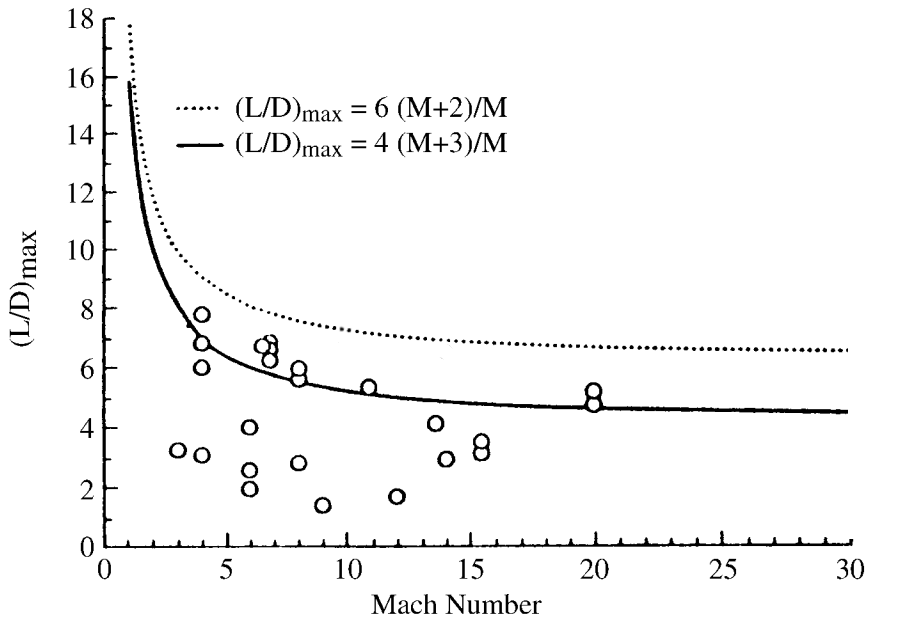
\includegraphics[width=0.55\textwidth]{figures/ld_limit.png}
    \caption{Maximum lift-to-drag ratio comparison for hypersonic vehicles. Conventional vehicles (circles) approach the solid line. Only waveriders can improve upon this; their aerodynamic efficiency approaches the dashed line. Adapted from \citep{Anderson:2019}.}
    \label{fig:ld_limit}
\end{figure}

In this section, we describe our approach to generating our waverider geometry. It consists of three major steps: (1) solving the inviscid flowfield around a shock-generating cone via the Taylor-Maccoll equations, (2) defining the trailing edge curve and projecting it onto the shock cone to obtain the leading edge, and (3) tracing streamlines from the leading edge to the trailing edge to carve out the upper and lower surfaces. Note that the algorithm proposed in this section largely follows that described by~\citep{Jones:1968}, and builds on the partial Python implementation provided by\ \citep{Zhou:2025}. Unlike conventional implementations, we parametrize the waverider upper trailing edge rather than its leading edge, allowing for greater control over the shape of the cabin. This helps create geometries that can satisfy necessary volume constraints.

\begin{figure}[htb!]
    \centering
    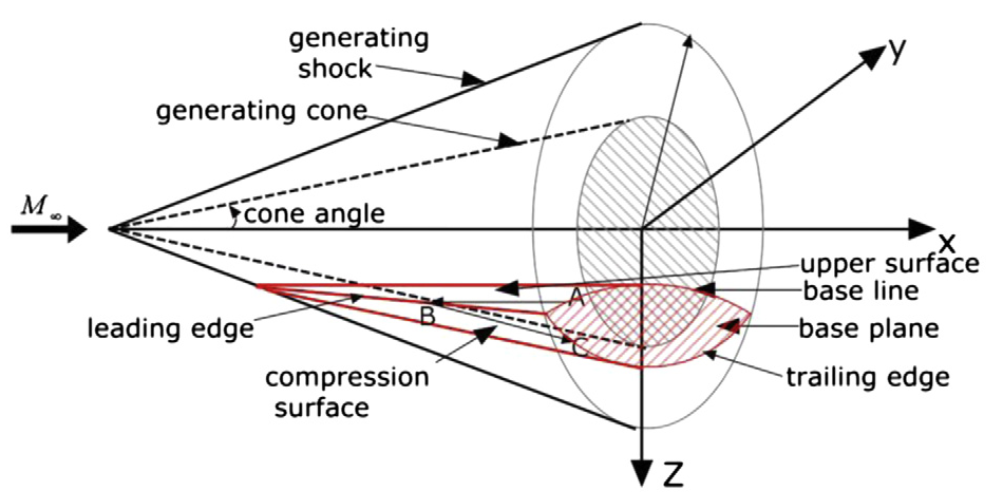
\includegraphics[width=0.55\textwidth]{figures/conical_waverider.png}
    \caption{Schematic of the cone-derived waverider geometry generation algorithm. The shock-generating cone is shown in black dashed lines, with the shock surface in solid lines. The waverider geometry is in red. The trailing edge (TE) is defined in the base plane $x=L$ and parameterized by $R_{1,\mathrm{frac}}$, $W_{\mathrm{frac}}$, and $n$. The leading edge (LE) is obtained by projecting the TE points radially inward along the shock cone surface. The lower surface is generated by tracing streamlines from the LE to the TE, while the upper surface is a ruled flat top. Reproduced from~\citep{Liu:2013}.}\label{fig:geometry}
\end{figure}

\subsection{Inviscid flow around a shock-generating cone}
Cone-derived waveriders are generated on the axisymmetric conical shock surface (with half-angle $\beta$) produced by a sharp-nosed cone (with half-angle $\theta_c$ and length $L$). This choice is convenient as the shock geometry and inviscid flowfield behind the shock are well-characterized via the oblique shock relations and the Taylor-Maccoll equations~\citep{Maccoll:1937}, respectively. These latter are a set of ODEs governing the flow in the conical region between the shock and the body cone, which exploit the self-similar (conical) nature of the flowfield --- all flow properties depend only on the polar angle $\theta$ measured from the cone axis. Ahead of the shock, the flowfield is simply the free-stream flow.

\subsubsection{Shock-jump relations}
For an oblique shock, the relationship between $\beta,M_\infty$, and $\theta_c$ is given by the $\theta-\beta-M$ relation:
\begin{equation}
    \tan\theta_c = 2\cot\beta \,
    \frac{M_\infty^2 \sin^2\!\beta - 1}{M_\infty^2\!\left(\gamma + \cos 2\beta\right) + 2}.
    \label{eq:theta_beta_M}
\end{equation}
The normal component of the upstream Mach number is $M_{n1}=M_\infty\sin\beta$ and the post-shock normal Mach number is given by the Rankine-Hugoniot jump conditions:
\begin{equation}
    M_{n2}^2 = \left(M_{n1}^2 + \dfrac{2}{\gamma-1}\right){\left(\dfrac{2\gamma}{\gamma-1}M_{n1}^2 - 1\right)}^{-1}.
    \label{eq:Mn2}
\end{equation}
The total post-shock Mach number follows from the geometry of the shock:
\begin{equation}
    M_2 = \frac{M_{n2}}{\sin(\beta - \theta_c)}.
    \label{eq:M2}
\end{equation}

\subsubsection{Taylor-Maccoll conical flow}
For calorically-perfect, steady, inviscid, isentropic flow about an axisymmetric cone with a conical structure, the velocity field in spherical coordinates $(r, \theta, \phi)$ reduces to $\mathbf{V} = V_r(\theta)\,\hat{r} + V_\theta(\theta)\,\hat{\theta}$. In the Taylor-Maccoll formulation, the velocity is non-dimensionalized by the maximum attainable speed, \textit{i.e.,} $V'=V/V_{\max}$, which corresponds to complete conversion of enthalpy to kinetic energy in an adiabatic process:
\begin{equation}
    V_{\max} = \sqrt{2 c_p T_0} = \sqrt{\frac{2 \gamma R T_0}{\gamma - 1}},
    \label{eq:Vmax}
\end{equation}
where $T_0=T_\infty\!\left(1 + \tfrac{\gamma-1}{2}M_\infty^2\right)$, and is in turn related to the local Mach number through the energy equation:
\begin{equation}
    \frac{1}{2} V'^2 + \frac{1}{\gamma - 1}\frac{a^2}{V_{\max}^2} = \frac{1}{2}
    \quad\Longrightarrow\quad
    V' = {\left(1 + \frac{2}{(\gamma-1)M^2}\right)}^{-1/2}
    \label{eq:Vprime}
\end{equation}
where $a$ is the local speed of sound.\\

Based on the axisymmetric, steady, irrotational (and constant entropy, via Crocco's theorem) nature of the flow behind the shock, the Euler equations reduce to the following non-dimensional governing equation~\citep{Maccoll:1937}:
\begin{equation}
    \frac{\gamma-1}{2}
    \left(1 - V'^2_r - V'^2_\theta\right)
    \left(2V'_r + V'_\theta\cot\theta + \frac{\mathrm{d}V'_\theta}{\mathrm{d}\theta}\right)
    - V'_\theta\left(V'_r V'_\theta + V'_\theta\frac{\mathrm{d}V'_\theta}{\mathrm{d}\theta}\right) = 0.
    \label{eq:TM_raw}
\end{equation}
Introducing $A = V'_r$ and $A' = \mathrm{d}V'_r/\mathrm{d}\theta$ (the irrotationality condition for a conical flow gives $V'_\theta = A'$, so that $\mathrm{d}V'_\theta/\mathrm{d}\theta = A''$), the equation can be rewritten as an explicit second-order ODE for $A$:
\begin{equation}
    A'' = \frac{A\,A'^2 - \dfrac{\gamma-1}{2}(1-A^2-A'^2)\!\left(2A + \dfrac{A'}{\tan\theta}\right)}
              {\dfrac{\gamma-1}{2}(1-A^2-A'^2) - A'^2}\label{eq:TM}
\end{equation}
This is split into the first-order system:
\begin{equation}
    \frac{\mathrm{d}}{\mathrm{d}\theta}
    \begin{pmatrix} A \\ A' \end{pmatrix} =
    \begin{pmatrix} A' \\ A'' \end{pmatrix}
\end{equation}

We solve this system by integrating inward from the shock surface $\theta = \beta$, where initial conditions are set by the oblique-shock solution:
\begin{align}
    V'_{r,i} &= V' \cos(\beta - \theta_c)\label{eq:Vri} \\
    V'_{\theta,i} &= -V' \sin(\beta - \theta_c),\label{eq:Vthetai}
\end{align}
toward the body cone at $\theta=\theta_c$. The body cone requires the streamlines to lie on the cone surface, \textit{i.e.,}\ $V'_\theta = A' = 0$. The ODE is solved with \texttt{scipy.integrate.solve\_ivp} using the Runge-Kutta 4,5 (RK45) method. This fully determines the flowfield around the generating cone.

\subsection{Determination of trailing and leading edge profiles}\label{sec:LE}

The \textbf{trailing edge (TE)} lies in the base plane $x = L$. We define it via three parameters: $R_\text{1,frac}$, $W_\text{frac}$, and $n$, such that any valid combination of these parameters results in a physically meaningful trailing-edge curve: one that remains inside the shock circle of radius $R_s = L\tan\beta$, is smooth, and remains below the cone axis. The parameters are defined as
\begin{align}
    R_1 &= R_{1,\mathrm{frac}}\,R_s, & y_{\mathrm{up}} &= W_{\mathrm{frac}}\,R_s,
\end{align}
with bounds $0.20 \le R_{1,\mathrm{frac}} \le 0.85$ and $0.25 \le W_{\mathrm{frac}} \le 0.85$. We define a gap function in squared-radius form,
\begin{equation}
    g(y) = (R_s^2 - R_1^2)\,\left(1 - \frac{y^2}{y_{\mathrm{up}}^2}\right)^{n}
    \quad\text{for}\quad |y| \le y_{\mathrm{up}},
\end{equation}
where $n = n_{\mathrm{shape}}$ (bounded to $0.6 \le n \le 10$) controls the roundness.  The TE curve is then
\begin{equation}
    z_{\mathrm{TE}}(y) = -\sqrt{R_s^2 - y^2 - g(y)},
    \label{eq:TE}
\end{equation}
which enforces $z_{\mathrm{TE}}(0) = -R_1$ and $z_{\mathrm{TE}}(y_{\mathrm{up}}) = -\sqrt{R_s^2 - y_{\mathrm{up}}^2}$ so the curve meets the shock circle at the tip.  Larger $n_{\mathrm{shape}}$ makes the tip tangent to the shock; $n_{\mathrm{shape}} < 1$ produces a sharper tip. An example of the trailing edge curve is shown in~\cref{fig:TE}.

\begin{figure}[htb!]
    \centering
    
\includegraphics[width=0.45\textwidth]{optimized_inviscid/baseplane.png}
    \caption{Example trailing edge curve for $M_\infty=6,\beta=13.791^\circ,R_{1,\mathrm{frac}}=0.348,W_{\mathrm{frac}}=0.605$, and $n=4.215$. The shock circle is shown for context.}\label{fig:TE}
\end{figure}

The \textbf{leading edge (LE)} is obtained by projecting every point on the TE curve radially {inward} along the shock cone surface.  For a point $(y, z) = (y_{\mathrm{TE}}, z_{\mathrm{TE}})$ in the base plane, the projection maintains the same azimuthal direction while scaling the axial coordinate to keep the point on the cone.  The radial distance from the cone axis is $\rho = \sqrt{y^2 + z^2}$; because the shock cone satisfies $\rho = x\tan\beta$, the axial coordinate of the LE is:
\begin{equation}
    X_{\mathrm{LE}} = L\left(1 - \frac{R_s - \rho}{R_s}\right)
                    = \frac{L\,\rho}{R_s}
    \label{eq:LE_x}
\end{equation}
with $Y_{\mathrm{LE}} = y_{\mathrm{TE}}$ and $Z_{\mathrm{LE}} = z_{\mathrm{TE}}$.

\subsection{Generation of the waverider surfaces via streamline tracing}\label{sec:streamline}

The full 3D waverider surface is generated by tracing streamlines in the conical flowfield. The upper surface is designed as a ruled surface swept from the leading edge straight to the trailing edge at constant $(y, z)$ --- a flat top that sees only the freestream. Note that an improvement could be made by instead allowing for a mild expansion along the upper surface, which would reduce pressure and allow for slightly more lift; this has been considered in the literature, but as it results in only a few percent improvement in $L/D$~\citep{Bowcutt:1986}, we neglect it as a second-order consideration. To compute the lower surface, streamlines are seeded just under the leading edge, and each is traced inward until it intersects the base plane. A streamline in the conical flowfield satisfies:
\begin{equation}
    \frac{\mathrm{d}r}{\mathrm{d}\theta} = r\,\frac{V'_r(\theta)}{V'_\theta(\theta)}
    \label{eq:streamline}
\end{equation}
where $V'_r(\theta)$ and $V'_\theta(\theta)$ are provided by the Taylor-Maccoll solution. Equation~(\ref{eq:streamline}) is solved via forward Euler.

\begin{figure}[htb!]
    \centering%
    
\includegraphics[width=0.75\textwidth]{optimized_inviscid/streamlines.png}
    \caption{Example streamline tracing from the leading edge to the trailing edge, for $M_\infty=6,\beta=13.791^\circ,R_{1,\mathrm{frac}}=0.348,W_{\mathrm{frac}}=0.605$, and $n=4.215$.}\label{fig:streamlines}
\end{figure}

Starting from $(r_0, \theta_0)$ at the shock surface, successive
points are computed as:
\begin{equation}
    r_{i+1} = r_i + \frac{V'_r(\theta_i)}{V'_\theta(\theta_i)}\,r_i\,\Delta\theta
    \label{eq:euler}
\end{equation}
where $\Delta\theta = \theta_{i+1} - \theta_i < 0$. Integration stops when the streamline crosses the base plane $x = L$, \textit{i.e.,}\ when $r_i\cos\theta_i < L \leq r_{i+1}\cos\theta_{i+1}$. At that crossing a linear interpolation gives the precise intersection point. The interpolated $z$-coordinate is:
\begin{equation}
    z_k^* = \cos\phi_k\,\left[
        \frac{r_{i+1}\sin\theta_{i+1} - r_i\sin\theta_i}
             {r_{i+1}\cos\theta_{i+1} - r_i\cos\theta_i}\,L
        + r_i\sin\theta_i
        - r_i\cos\theta_i\,
          \frac{r_{i+1}\sin\theta_{i+1} - r_i\sin\theta_i}
               {r_{i+1}\cos\theta_{i+1} - r_i\cos\theta_i}
    \right],\label{eq:interp}
\end{equation}
where the azimuthal angle of the plane is $\phi_k=-\arctan\!\left(\frac{Y_k}{Z_k}\right)$. From $z_k^*$ the intersection spherical coordinates are recovered:
\begin{gather}
    r_k^* = \sqrt{(z_k^*/\cos\phi_k)^2 + L^2},\qquad
    \theta_k^* = \arctan\!\left(\frac{z_k^*/\cos\phi_k}{L}\right).
\end{gather}
\cref{fig:streamlines} shows an example of the streamlines traced from the leading edge to the trailing edge for the same case as~\cref{fig:TE}, which form the lower surface of the waverider. The upper surface is generated by connecting each point on the leading edge to its corresponding point on the trailing edge via a straight line, forming a ruled surface. Finally, a computational mesh (panelization) is generated by seeding nodes along each streamline at fixed intervals, then connecting those nodes to triangulate the upper and lower surfaces.

\subsection{Algorithm summary}\label{sec:algorithm}
\begin{enumerate}[label=\textbf{Step \arabic*.}, leftmargin=*, itemsep=4pt]
    \item \textbf{Input:} Read freestream conditions $(M_\infty,\gamma)$, generating shock parameters $(\beta,L)$, and the trailing edge description $(R_{1,\mathrm{frac}}, W_{\mathrm{frac}}, n)$.
    \item \textbf{Oblique shock:} Solve \cref{eq:theta_beta_M,eq:M2} to obtain $M_2$, $\theta$; form initial conditions $(V'_{r,i}, V'_{\theta,i})$ via \cref{eq:Vri,eq:Vthetai}.
    \item \textbf{Taylor-Maccoll:} Integrate \cref{eq:TM} from $\theta = \beta$ inward with RK45 until $V'_\theta = 0$; record body-cone angle $\theta_c$.
    \item \textbf{Trailing edge:} Evaluate the admissible back-face curve \cref{eq:TE} over $|y| \le y_{\mathrm{up}}$; compute break-point array.
    \item \textbf{Leading edge:} Project TE points onto shock cone via \cref{eq:LE_x}.
    \item \textbf{Streamline tracing:} For each of $N_l$ seed points on the leading edge:
          \begin{enumerate}[label=\alph*.]
              \item compute plane azimuth $\phi$,
              \item re-integrate Taylor-Maccoll on uniform $\theta$-grid,
              \item Euler-march \cref{eq:euler} until base-plane crossing,
              \item interpolate exact intersection \cref{eq:interp},
              \item convert to Cartesian coordinates.
          \end{enumerate}
    \item \textbf{B-spline:} Fit smooth curve through base-plane endpoints.
    \item \textbf{Upper surface:} Ruled lines from LE break points to TE.
    \item \textbf{Mesh generation:} Points are seeded along the streamlines and connected into triangles.\@
\end{enumerate}

Example waverider geometries generated by this algorithm for fixed $M_\infty,L,\beta$ are shown in~\cref{fig:waveriders}, showing that diverse shapes can be generated by varying the input parameters.

\begin{figure}[p]
    \centering
    \includegraphics[width=0.75\textwidth]{te_sweep/geometry_grid_13.png}
    \caption{Example waverider geometries generated by our algorithm for different input parameters, using $M_\infty=6,\beta=13^\circ,\gamma=1.4,L=20$ m. Note that $L/D$ ratios reported above consider inviscid effects only; see the following section for details.}\label{fig:waveriders}
\end{figure}

% ==========================================================================
% \FloatBarrier%
\section{Aerothermodynamics \& waverider geometry optimization}\label{sec:aerothermodynamics}
In this section, we describe our approach to computing the aerodynamic characteristics of an ideal (sharp) waverider, including pressure (\cref{sec:inviscid}) and viscous forces (\cref{sec:bl}). Then, we account for non-idealities arising from necessary blunting of the leading edge (\cref{sec:blunting}) and viscous interaction (\cref{sec:interaction}). We combine these analyses to compute the mean pressure coefficient, total lift-to-drag ratio, and maximum skin friction and heating rates. Note that we do not account for wake (base) drag, as this is beyond the scope of the present effort. Finally, we describe the methods used to optimize the waverider geometry given design objectives and constraints (\cref{sec:optimization}). The final optimized geometry and its performance metrics are given at the end of the section.

\subsection{Pressure distribution and inviscid forces}\label{sec:inviscid}

By design, the \textbf{upper surface} of the waverider is a ruled flat top that sees only the undisturbed freestream. Though the blunt edge of a real waverider would produce a weak detached bow shock and a more complex flowfield, we neglect this consideration in the present analysis. Thus, we take the pressure coefficient over the upper surface to be zero ($C_p^\text{upper} = 0$), and assume that it contributes no pressure drag (but that it will contribute to the skin friction drag, which is calculated in the next section).

Conversely, the pressure coefficient on the \textbf{lower surface} is non-zero, and is computed from the Taylor-Maccoll solution. Because the lower surface is a stream surface, each streamline lies in an azimuthal plane, and its boundary-layer-edge properties are functions of the polar angle $\theta$ from the cone axis. For each point on a streamline, we look up $V'(\theta)^2 = V'^2_r + V'^2_\theta$ and compute the dimensional quantities. The stagnation temperature and pressure are constant in the post-shock region; this gives, with freestream $T_\infty$ and $p_\infty$:
\begin{gather}
    u = V'(\theta)\sqrt{2\gamma R T_0/(\gamma-1)},\quad
    T = T_0\!\left(1 - V'^2(\theta)\right), \quad
    M = u / \sqrt{\gamma R T},\quad
    p = p_{02}\,{(1-V'^2(\theta))}^{\gamma/(\gamma-1)},
\end{gather}
where $p_{02}$ is the post-shock stagnation pressure:
\begin{equation}
    \frac{p_2}{p_\infty} = \frac{2\gamma M_{n1}^2 - (\gamma-1)}{\gamma+1}, \qquad
    \frac{p_{02}}{p_\infty} = \frac{p_2}{p_\infty}\left(1 + \tfrac{\gamma-1}{2}M_2^2\right)^{\gamma/(\gamma-1)}.
\end{equation}
The pressure coefficient follows:
\begin{equation}
    C_p^\text{lower} = \frac{p/p_\infty - 1}{\tfrac{\gamma}{2}M_\infty^2}
    = \frac{2}{\gamma M_\infty^2}\left[\left(\dfrac{p_{02}}{p_\infty}\right)(1-V'^2)^{\gamma/(\gamma-1)} - 1\right]
\end{equation}

To integrate the pressure forces, the lower surface is panelized into triangles with area $\mathrm{d}A$ and outward unit normal $\hat{\mathbf{n}}$.  The pressure force on each panel is integrated in coefficient form as
\begin{equation}
    \mathrm{d}\mathbf{C}_F = -C_p\,\hat{\mathbf{n}}\,\frac{\mathrm{d}A}{S_{\mathrm{ref}}},
\end{equation}
so the total force coefficient vector is $\mathbf{C}_F = \sum \mathrm{d}\mathbf{C}_F$.  The reference area is the
planform (projection) of the lower surface onto the $x$-$y$ plane,
\begin{equation}
    S_{\mathrm{ref}} = \sum\!\left|\frac{1}{2}
    \left[(x_1-x_0)(y_2-y_0) - (y_1-y_0)(x_2-x_0)\right]\right|,
\end{equation}
using the projected triangle vertices $(x_i,y_i)$. The coefficient components are reported as $C_L = C_{F,z}$, $C_{D_p} = C_{F,x}$, and ${(L/D)}_\text{inviscid} = C_L/C_{D_p}$.

\subsection{Viscous shear contributions via boundary layer integration}\label{sec:bl}
To estimate viscous drag on the waverider surface, we use the laminar compressible integral boundary-layer method of Walz~\citep{Walz:1969}, exactly following the implementation reported by Bowcutt in his seminal paper on viscous-optimized waverider design~\citep{Bowcutt:1986,Bowcutt:1987}. The method assumes that the boundary layer is locally 2D in azimuthal planes, that it is steady, laminar, and attached, that it is in a continuum regime, and furthermore that it develops from a sharp edge. We obtain the boundary layer edge conditions \(\{u_e, M_e, \rho_e, T_e\}\) from the external inviscid flow as described above, then march the boundary layer downstream by solving a coupled pair of first-order ordinary differential equations along each streamline on the boundary-layer edge. The model accounts for compressibility, wall-temperature effects, and streamwise pressure-gradient effects through the prescribed edge flow. Flow separation or transition to turbulence is not considered. An isothermal wall at $T_w$ is assumed; radiative equilibrium is not modeled (Bowcutt suggests that this is a reasonable assumption away from the stagnation point).

The two governing equations are the integral momentum equation and the integral mechanical-energy equation, where $s$ is a coordinate along the boundary-layer-edge streamline, and $y$ is the coordinate normal to the surface:
\begin{gather}
    \frac{\mathrm{d}Z}{\mathrm{d}s}
    + \frac{1}{u_e}\frac{\mathrm{d}u_e}{\mathrm{d}s}\,F_1\,Z
    - F_2 = 0,\qquad
    \frac{\mathrm{d}W}{\mathrm{d}s}
    + \frac{1}{u_e}\frac{\mathrm{d}u_e}{\mathrm{d}s}\,F_3\,W
    - \frac{F_4}{Z} = 0,
\end{gather}
where $\delta_1$, $\delta_2$, and $\delta_3$ are, respectively, the displacement, momentum, and energy thicknesses of the boundary layer, and $Z$ and $W$ are dimensionless integration variables; these are defined as:
\begin{gather}
    Z = \delta_2\left(\frac{\rho_e u_e \delta_2}{\mu_w}\right)
    = \frac{\rho_e u_e \delta_2^2}{\mu_w},\qquad
    W = \frac{\delta_3}{\delta_2},\\[4pt]
    \delta_1 = \int_0^\delta
    \left(1-\frac{\rho u}{\rho_e u_e}\right)\,\mathrm{d}y,\qquad
    \delta_2 = \int_0^\delta
    \frac{\rho u}{\rho_e u_e}
    \left(1-\frac{u}{u_e}\right)\,\mathrm{d}y,\qquad
    \delta_3 = \int_0^\delta
    \frac{\rho u}{\rho_e u_e}
    \left(1-\frac{u^2}{u_e^2}\right)\,\mathrm{d}y,
\end{gather}
where ${(\cdot)}_w$ denotes evaluation at the wall. The empirical closures for these equations (copied directly from the textbook,~\cite{Walz:1969}) are:
\begin{gather}
    F_1 = 3 + 2H - M_e^2
    + n\,
    \frac{\dfrac{1}{\mu_w}\dfrac{\mathrm{d}\mu_w}{\mathrm{d}s}}
        {\dfrac{1}{u_e}\dfrac{\mathrm{d}u_e}{\mathrm{d}s}},
    \qquad
    n =
    \begin{cases}
    0, & T_w = \text{constant},\\
    1, & T_w \neq \text{constant},
    \end{cases}\\[6pt]
    F_2 = \frac{2a}{b},\qquad
    F_3 = 1 - H + r(\gamma-1)M_e^2\left(1-\frac{\widetilde{\theta}}{W}\right),\qquad
    F_4 = \frac{2\beta - aW}{b},
\end{gather}
and
\begin{gather}
    H = \frac{\delta_1}{\delta_2}
    = b\,H_{12}
    + r\,\frac{\gamma-1}{2}\,M_e^2\left(W-\widetilde{\theta}\right),\\[4pt]
    a = 1.7261\left(W^\ast - 1.515\right)^{0.7158},\qquad
    b = \frac{\delta_2^{(u)}}{\delta_2}
    = 1 + r\,\frac{\gamma-1}{2}\,M_e^2
    \left(W-\widetilde{\theta}\right)\left(2-W\right),\\[4pt]
    r = \sqrt{\Pr},\qquad
    \widetilde{\theta} =
    \frac{T_{aw}(s)-T_w(s)}{T_{aw}(s)-T_e(s)},\qquad
    \beta = \beta^{(u)}\,\chi,
\end{gather}
and
\begin{gather}
    H_{12} = 4.0306 - 4.2845\left(W^\ast - 1.515\right)^{0.3886},\qquad
    T_{aw} = T_e + \frac{r\,u_e^2}{2c_p},\quad
    W^\ast = \frac{\delta_3^{(u)}}{\delta_2^{(u)}} = \frac{W}{\psi},\label{eqn:W}\\[4pt]
    \psi = 1 + \frac{(\psi_{12}-1)M_e^2}
    {M_e^2 + \psi_{12}^{-1}/\psi_0},\qquad
    \psi_{12} =
    \frac{2-\delta_1^{(u)}/\delta}{W^\ast}\,\widetilde{\theta}
    +
    \frac{1-\delta_1^{(u)}/\delta}{W^\ast g}\,(1-\widetilde{\theta}),\\[4pt]
    \psi_0 = 0.0144\,(2-W^\ast)\,(2-\widetilde{\theta})^{0.8},\qquad
    \frac{\delta_1^{(u)}}{\delta}
    = 0.420 - \left(W^\ast - 1.515\right)^{0.424\,W^\ast},\\[4pt]
    g = 0.324 + 0.336\left(W^\ast - 1.515\right)^{0.555},\qquad
    \beta^{(u)} = 0.1564 + 2.1921\left(W^\ast - 1.515\right)^{1.70},\\[4pt]
    \chi =\left\{
    1 + r\,\frac{\gamma-1}{2}\,M_e^2
    \left[
    1.16\,W^\ast - 1.072 - \widetilde{\theta}(2W^\ast - 2.581)
    \right]
    \right\}^{0.7}
    \left\{
    1 + r\,\frac{\gamma-1}{2}\,M_e^2(1-\widetilde{\theta})
    \right\}^{-0.7}.
\end{gather}
Finally, wall viscosity $\mu_w(T_w)$ is given by Sutherland's law,
\begin{gather}
    \mu(T) = \mu_0\!\left(\frac{T}{T_0^{\mu}}\right)^{3/2}
              \frac{T_0^{\mu} + S}{T+S},
    \quad \mu_0 = 1.716\!\times\!10^{-5}\ \mathrm{Pa\,s},\
    T_0^{\mu}=273.15\ \mathrm{K},\ S=110.4\ \mathrm{K}.
\end{gather}

At the leading edge $s=0$ the boundary layer has zero thickness, so $Z\to 0$ is singular for the $W$-equation.  We start the integration at a small $s_0>0$ from the local self-similar (zero pressure-gradient) state. Setting $\mathrm{d}W/\mathrm{d}s=0$ in the $W$-equation with $\mathrm{d}u_e/\mathrm{d}s=0$ gives the algebraic fixed point $W = 2\beta/a$.  With~\cref{eqn:W} this is iterated together with the $W\!\leftrightarrow\!W^\ast$ inversion until self-consistent (the incompressible Blasius value $W^\ast \approx 1.572$ is used as the seed). The matching $Z$ is then $Z(s_0) = (2a/b)\,s_0$, which is the linear Blasius-like growth.

\subsubsection{Numerical integration along streamlines}
For each streamline, the integration is performed as follows:
\begin{enumerate}[leftmargin=*]
  \item The streamline is sampled to a uniform grid in arc length $s$.
  \item $\bigl(u_e,T_e,M_e,\rho_e,\mu_w,\widetilde{\theta}\bigr)$ are tabulated at each station; linear interpolants are built to evaluate them between stations.
  \item The coupled system $\bigl(Z(s),W(s)\bigr)$ is integrated with RK45 from the \texttt{scipy.integrate.solve\_ivp} package.
  \item At every RHS evaluation, given the current compressible $W$ and the local edge state, the implicit relation~\eqref{eqn:W} is solved for the self-consistent $W^\ast$ via \texttt{scipy.optimize.brentq}, then $a,\,b,\,H_{12},\,H,\,\beta^{(u)},\,\chi,\,\beta$ and the four coefficients $F_1,F_2,F_3,F_4$ are evaluated.
\end{enumerate}
The momentum thickness, wall shear, and skin-friction coefficient are recovered post-integration by:
\begin{equation}
    \delta_2 = \sqrt{\frac{Z\,\mu_w}{\rho_e u_e}},\qquad
    \tau_w   = \frac{a\,\mu_w u_e}{\delta_2},\qquad
    c_f      = \frac{2\tau_w}{\rho_e u_e^2}.
    \label{eq:tauw}
\end{equation}

\subsubsection{Skin-friction drag integration over the waverider surfaces}
On both surfaces, each streamline represents a strip of the wetted surface; strip width $w(s)$ is approximated by the half-distance to each neighbouring streamline at the same fractional arc length (with a single-neighbour doubling at the outermost streamlines).  The streamwise friction force on the strip is
\begin{equation}
    F_{x,k} \;=\; \int_0^{s_{\mathrm{TE}}}
        \tau_w(s)\,\bigl(\mathrm{d}x/\mathrm{d}s\bigr)\,w(s)\,\mathrm{d}s,
\end{equation}
evaluated by the trapezoidal rule.  The total friction-drag coefficient sums the contributions from both surfaces, each doubled to account for the mirrored half:
\begin{equation}
    C_{D_f}
    \;=\; \frac{2}{q_\infty S_{\mathrm{ref}}}
    \!\left(
        \sum_{k=1}^{N_l} F_{x,k}^{\mathrm{lower}}
      + \sum_{k=1}^{N_{up}} F_{x,k}^{\mathrm{upper}}
    \right),
    \qquad
    C_{D_f} = C_{D_f}^{\mathrm{lower}} + C_{D_f}^{\mathrm{upper}},
\end{equation}
with $S_{\mathrm{ref}}$ the planform projection of the lower surface.


\subsection{Aerothermal heating and the blunt leading-edge correction}\label{sec:blunting}

The cone construction produces an aerodynamically sharp leading edge, which is unphysical: stagnation-point convective heating scales as $1/\sqrt{R_n}$ and would be unbounded. A finite blunting radius $R_n$ is required to keep the surface temperature below a chosen material limit $T_{\text{allow}}$. The degree of bluntness must be selected such that maximum expected aerothermal heating is manageable, but should be as small as possible to preserve the aerodynamic performance of the waverider.

The effects of blunting can be significant: local pressure drag is increased, the shock wave may `leak' over the leading edge to the upper surface, decreasing lift, and a bow shock may form at some standoff distance from the leading edge. Blunting also increases the potential for flow separation and transition to turbulence, which in turn increases drag and heating. That said, for sufficiently performant high-temperature thermal protection system materials, and assuming that a hot aerostructure is employed, the required blunting radius may be very small (at most a few centimeters for the present design space,~\cite{Bowcutt:1986,Anderson:2019,Peters:2024}), and thus the vehicle may be considered `aerodynamically sharp' when considering the macroscopic flowfield. For this reason, we neglect most of the aforementioned effects in the present analysis. Nevertheless, even a small amount of blunting can induce significant localized drag (up to 8\% of total drag~\citep{Vanmol:1992}), which we do account for via a bluntness correction to the pressure distribution on the leading edge.

Determining the minimum required blunting radius requires an estimate of the aerothermal heating to the vehicle. In our present analysis, we consider a single uniform blunting radius based only on the worst-case heating at the stagnation point. A higher-fidelity analytical treatment of the blunted leading edge may involve allowing for a variable radius and computing heat flux and pressure distributions all along the leading edge, and indeed over the surface of the whole vehicle~\citep{Vanmol:1992}. However, modern non-equilibrium chemically-reacting CFD analysis of blunted waveriders overwhelmingly supports that heating away from the nose of the vehicle is orders of magnitude lower than the stagnation-point heating~\citep{Liu:2013}; and likewise that the flow is chemically-frozen away from the leading edge~\citep{Anderson:1992}. Our simplification is therefore conservative and should not meaningfully underestimate the required blunting radius.

In summary, we treat the blunt leading edge as a circular cylinder of radius $R_n$ swept along the streamline-derived leading edge curve. To determine $R_n$, we assume that the nose of the waverider is in radiative thermal equilibrium with its environment and that no active cooling is used; this gives a direct relationship between the blunting radius and the maximum surface temperature. We compute and add the inviscid pressure force contributions of the blunt leading edge to the sharp leading edge result from the previous sections via modified Newtonian impact theory. Since the blunted portions are leading edges, a boundary layer has not yet developed, and we do not account for viscous effects in the bluntness correction.

\subsubsection{Minimum blunting radius from aerothermal heating constraints}
Convective heating at the stagnation point is estimated from the Sutton-Graves correlation for air in chemical equilibrium~\citep{Sutton:1971}, which accounts for bow shock heating and exothermic chemical reactions at the stagnation point:
\begin{equation}
    \dot{q}_{\text{conv}} = k_{\text{SG}}\sqrt{\frac{\rho_\infty}{R_n}}\,V_\infty^{3},
    \qquad k_{\text{SG}} = 1.83 \times 10^{-4}\ \mathrm{W\,s^{3}\,kg^{-1/2}\,m^{-7/2}}.
    \label{eq:sutton_graves}
\end{equation}
This heating is balanced against radiative equilibrium with an emissivity $\varepsilon$ and Stefan-Boltzmann constant $\sigma$:
\begin{equation}
    \dot{q}_{\text{rad}} = \varepsilon\sigma\!\left(T_w^{4} - T_\infty^{4}\right).
    \label{eq:rad_eq}
\end{equation}
Setting $\dot{q}_{\text{conv}} = \dot{q}_{\text{rad}}$ at $T_w = T_{\text{allow}}$ and applying a safety factor $s_f \ge 1$ gives
\begin{equation}
    R_{n,\min}
    = \rho_\infty\!\left(
        \frac{s_f\,k_{\text{SG}}\,V_\infty^{3}}
                {\varepsilon\sigma\!\left(T_{\text{allow}}^{4}-T_\infty^{4}\right)}
        \right)^{2}.\label{eq:Rmin}
\end{equation}
The maximum allowable temperature, $T_{\text{allow}}$, and the emissivity $\varepsilon$ are material properties of the thermal protection system, and the safety factor $s_f$ accounts for uncertainties in the heating estimate and material properties. For a given material choice, \cref{eq:Rmin} gives a direct relationship between the blunting radius and the maximum expected aerothermal heating. This relationship is illustrated in~\cref{fig:blunting}.

\begin{figure}[htb]
    \centering%
    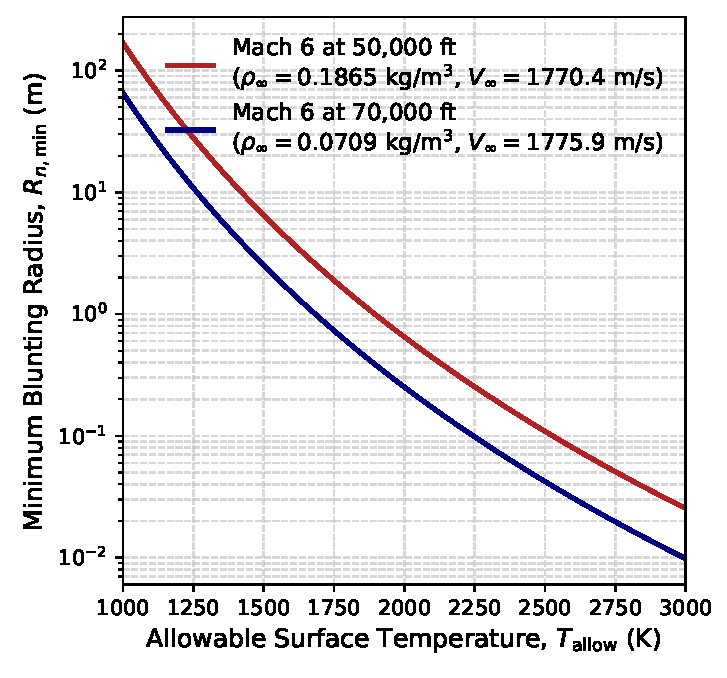
\includegraphics[width=0.5\textwidth]{blunting.pdf}
    \caption{Minimum blunting radius as a function of maximum allowable material surface temperature, for $\varepsilon=0.9,M_\infty=6,s_f=1.5$ at various altitudes, assuming Sutton-Graves stagnation point heating and a passively cooled material in radiative thermal equilibrium.}
    \label{fig:blunting}
\end{figure}

\subsubsection{Modified-Newtonian force along a swept leading edge}\label{sec:LE_newton}
To determine the contribution of the blunted leading edge to the overall aerodynamic forces, we apply modified Newtonian theory. At each point along the leading edge, the velocity  $\mathbf{u}_\perp$ and Mach number, $M_\perp$, perpendicular to the leading edge (normal to the local tangent) are computed as:
\begin{gather}
    \hat{\mathbf{u}}_\perp = \frac{\hat{\mathbf{u}}_\infty - \sin\Lambda\,\hat{\mathbf{t}}}{||\hat{\mathbf{u}}_\infty - \sin\Lambda\,\hat{\mathbf{t}}||},\qquad
    M_\perp = M_\infty\cos\Lambda,
\end{gather}
where $\sin\Lambda=\hat{\mathbf{t}}\!\cdot\!\hat{\mathbf{u}}_\infty$ is the local sweep angle between the leading edge tangent and the freestream direction, and $\hat{\mathbf{t}}$ is the local unit tangent vector. In the plane perpendicular to $\hat{\mathbf{t}}$, the cylinder cross-section is a circle of radius $R_n$, parameterised by an angle $\phi$ measured from the stagnation line.  The modified-Newtonian distribution is
\begin{equation}
    C_p(\phi) = C_{p,\max}(M_\perp)\,\cos^{2}\!\Lambda\,\cos^{2}\!\phi,
    \qquad |\phi| \le \pi/2 \text{ (windward)},
\end{equation}
and zero on the leeward side. $C_{p,\max}$ follows from the normal-shock stagnation-pressure construction:
\begin{equation}
    C_{p,\max}(M_\perp)
    = \frac{p_{02}/p_1 - 1}{\tfrac{1}{2}\gamma M_\perp^{2}},
    \label{eq:Cpmax}
\end{equation}
where $p_{02}/p_1$ is built from the standard normal-shock and isentropic relations applied to $M_\perp$. Integrating the pressure load $-C_p\,q_\infty\,R_n\,\hat{\mathbf{n}}\,\mathrm{d}\phi\,\mathrm{d}s$ over the windward half exploits $\int_{-\pi/2}^{\pi/2}\cos^{3}\phi\,\mathrm{d}\phi = 4/3$ and gives a closed-form resultant force per unit leading edge arc length,
\begin{equation}
    \frac{\mathrm{d}\mathbf{F}}{\mathrm{d}s}
    = \tfrac{4}{3}\,q_\infty\,R_n\,C_{p,\max}(M_\perp)\,\cos^{2}\!\Lambda\;\hat{\mathbf{u}}_\perp.
    \label{eq:LE_force}
\end{equation}
The transverse component (in the $\hat{\mathbf{t}}\!\times\!\hat{\mathbf{u}}_\perp$ direction) vanishes by symmetry of $\cos^{2}\!\phi$ about $\phi = 0$.

The leading-edge curve $\{(X_k,Y_k,Z_k)\}_{k=1}^{N}$ from \cref{sec:LE} is differenced to obtain segment tangents $\hat{\mathbf{t}}_k$ and arc lengths $\Delta s_k$.\@ \cref{eq:LE_force} is evaluated at every segment and summed,
\begin{equation}
    \mathbf{F}_{\text{LE}}
    \;=\; \sum_{k} \tfrac{4}{3}\,q_\infty\,R_n\,
        C_{p,\max}(M_{\perp,k})\,\cos^{2}\!\Lambda_k\;\hat{\mathbf{u}}_{\perp,k}\,\Delta s_k.
\end{equation}
Because the discretised leading edge spans the full vehicle ($y\in[-y_{\text{up}},+y_{\text{up}}]$) no symmetry doubling is required. The resultant lift- and drag-coefficient increments are
\begin{equation}
    \Delta C_L = \frac{F_{\text{LE},z}}{q_\infty S_{\text{ref}}},
    \qquad
    \Delta C_D = \frac{F_{\text{LE},x}}{q_\infty S_{\text{ref}}}.
\end{equation}
Finally, the total drag coefficient is $C_D = C_{D_p} + C_{D_f} + C_{D_B}$, and the total lift-to-drag ratio is $L/D = C_L / C_D$.

\subsection{Viscous interaction and Shock Wave-Boundary Layer Interaction (SWBLI)}\label{sec:interaction}
In the hypersonic regime, the immense aerodynamic heating and flow deceleration near the vehicle surface can cause the boundary layer to grow exceptionally thick, leading to viscous pressure interaction, which can significantly increase skin friction and heating rates. For our waverider, which relies on a perfectly tailored geometry to keep its bow shock attached exactly to its leading edge, a thick boundary layer can also push the shock wave outward, causing undesirable `leakage' of high-pressure air from the lower surface, further degrading lift~\citep{Anderson:2019}. A similarly important effect is shock wave-boundary layer interaction (SWBLI), which occurs when a shock wave impinges on the boundary layer, causing it to thicken and potentially separate. 

\begin{figure}[htb!]
    \centering
    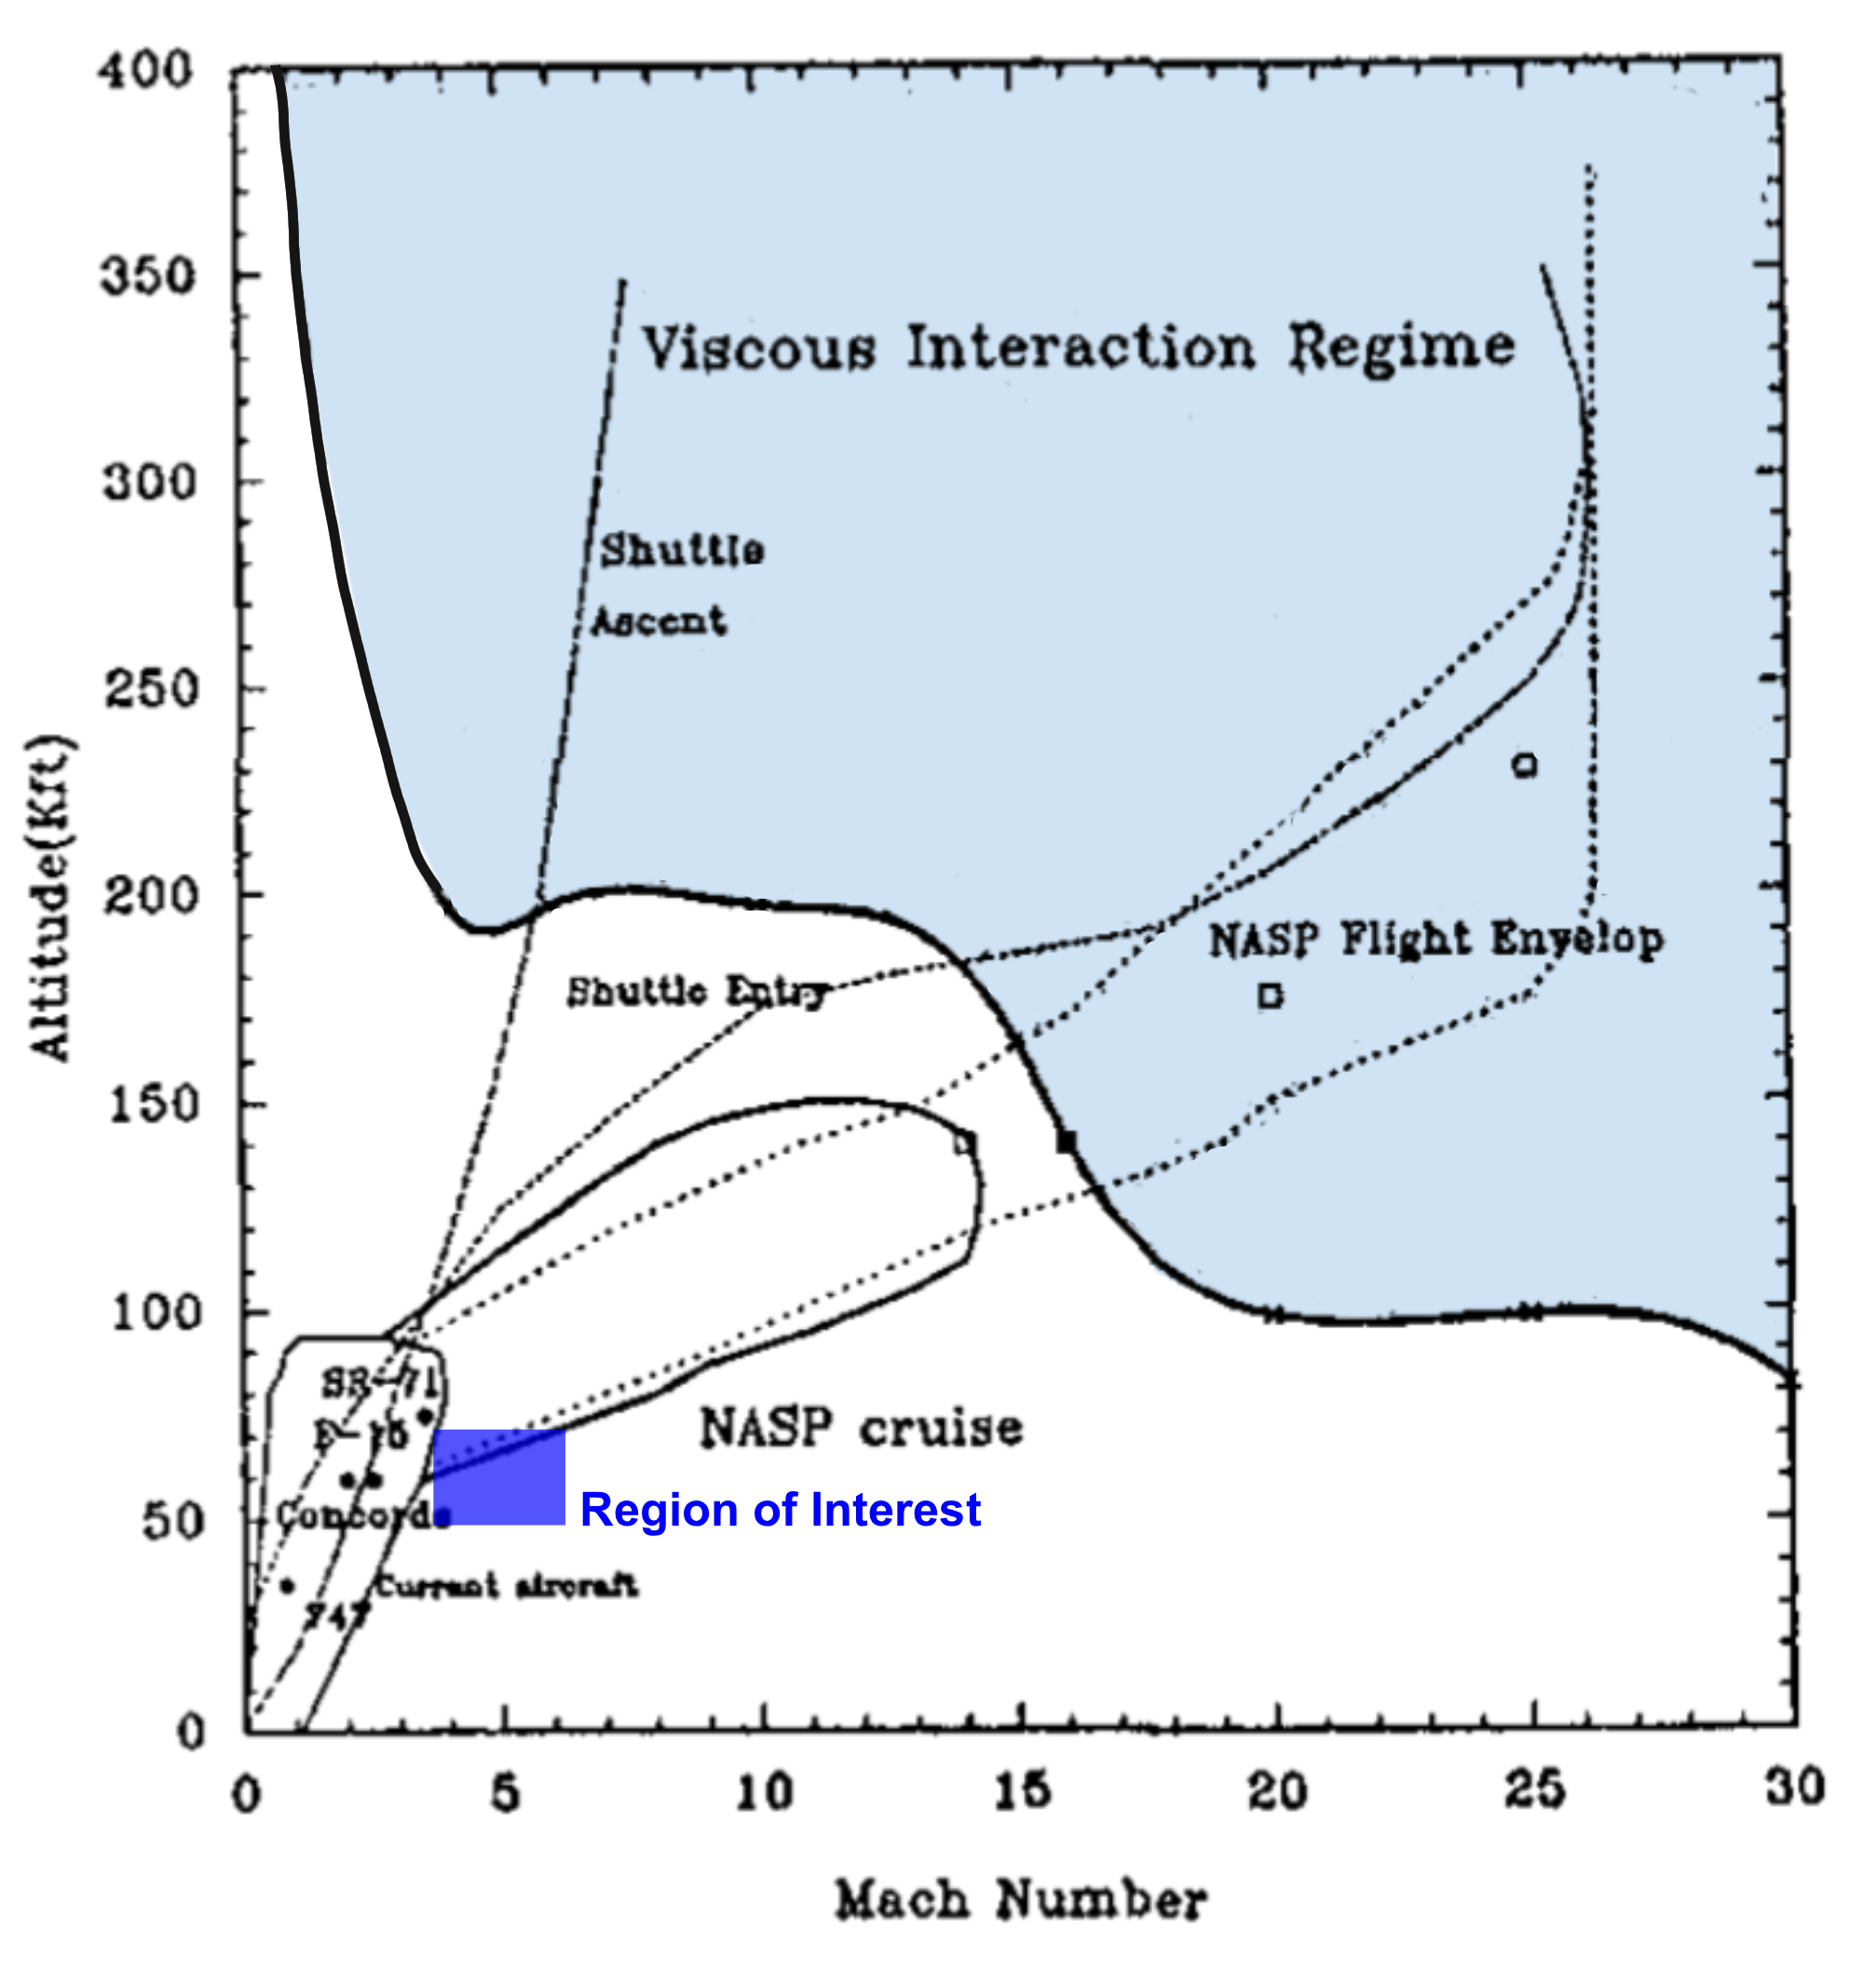
\includegraphics[width=0.45\textwidth]{figures/Chang1992.png}
    \caption{Notional velocity-altitude plot showing the region (light blue) where viscous interaction significantly influences $L/D$ ($>5\%$ change) for a 60-m hypersonic waverider. The region of interest for the present work (Mach 4 to 6, altitudes 50,000 to 70,000 ft) is indicated in dark blue; it is far outside the region of significant interaction. Adapted from~\citep{Anderson:1992,Anderson:2019}.}\label{fig:viscous_interaction}
\end{figure}

In the present work, we treat neither effect. Detailed exploration of the waverider design space by~\citep{Anderson:1992} shows that for a 60-meter-long hypersonic waverider, viscous pressure interactions have a significant influence (greater than 5\%) on $L/D$ only for certain Mach number-altitude combinations, highlighted in light blue on~\cref{fig:viscous_interaction}. The region of interest for the present work (Mach 4 to 6, altitudes 50,000 to 70,000 ft) is far outside the region of significant interaction, which justifies our neglect of viscous pressure interactions. As for the shock-wave-boundary layer interaction: by design, all shocks produced by our waverider are directed outward and away from the vehicle, or impinge on the vehicle exactly at the leading edge where the boundary layer thickness is zero, and so SWBLI is avoided. We are afforded the luxury of such a design because the practical engineering and manufacturing considerations that may lead to the necessary protrusions that would produce such impinging shocks (\textit{e.g.,} engine nacelles, cockpit windows, stabilizing fins, \ldots) are outside the scope of the present investigation. Nevertheless, we acknowledge that these effects can be significant and that they should be considered in a more comprehensive analysis.

\subsection{Constrained optimization of waverider geometry}\label{sec:optimization}
In~\cref{sec:geometry,sec:aerothermodynamics}, we established an algorithm for the geometric construction of the waverider and the methods for computing its aerothermodynamic performance. In this section, we seek to optimize the design parameters to maximize aerodynamic efficiency under cruise conditions, subject to the coupled geometric and thermal design constraints described in~\cref{sec:intro,sec:trajectory,sec:propulsion,sec:weight}. To achieve this, we perform a global optimization over all free geometric parameters ($L,\beta,R_{1,\text{frac}},W_{\text{frac}},n$).

\subsubsection{Determination of optimal airframe configuration}
Though most studies of waverider optimization seek to maximize the lift-to-drag ratio, $L/D$, this frequently drives the optimization toward thin geometries that are structurally inefficient and require a very high dry vehicle mass to meet payload capacity requirements. Instead, we choose the objective function:
\begin{gather}
    J(\mathbf{x})=V/(L/D)\propto W/(L/D)=T
\end{gather}
which minimizes thrust $T$ (and thus fuel) requirements in steady level flight. This penalizes inefficient shapes, thereby forcing the optimizer to balance aerodynamics and practical considerations.

The formal geometry optimization problem is posed as:
\begin{gather}
    \begin{aligned}
        \min_{\mathbf{x}} \quad & J(\mathbf{x}) = V(\mathbf{x})\cdot{\left(\frac{L}{D}(\mathbf{x})\right)}^{-1} \\
        \text{subject to} \quad & g_1(\mathbf{x}) = H_{\text{req}} - H(\mathbf{x}) \le 0 \\
        & g_2(\mathbf{x}) = A_{\text{req}} - A(\mathbf{x}) \le 0 \\
        & g_3(\mathbf{x}) = V_{\text{cabin}} + V_{\text{fuel}}(\mathbf{x}) - V(\mathbf{x}) \le 0 \\
        \text{with bounds} \quad & \mathbf{x}_\text{min} \le \mathbf{x} \le \mathbf{x}_\text{max}
    \end{aligned}
\end{gather}
where $\mathbf{x} = {[\beta, L, R_{1,\text{frac}}, W_{\text{frac}}, n]}^\top$ are the design variables, $J(\mathbf{x})$ is the objective function to minimize, and $g_i(\mathbf{x})$ are the constraint functions that must be satisfied. The bounds on the design variables are defined by $\mathbf{x}_\text{min}$ and $\mathbf{x}_\text{max}$: the shock-angle bounds are set from the Mach angle,\ $\beta_{\min} = \max\left(\sin^{-1}(1/M_\infty) + 0.5^{\circ},\,1^{\circ}\right)$ and $\beta_{\max} = 18^{\circ}$, while the trailing-edge bounds are taken from their admissible ranges (see~\cref{sec:LE}).

To solve the optimization problem, we use a differential evolution algorithm~\citep{Storn:1997} from the SciPy library, \texttt{scipy.optimize.differential\_evolution}, which is a powerful global optimization method that does not require gradient information and is well-suited for non-convex problems with multiple local minima. To enforce the geometric constraints, we use a predictor-corrector approach within the optimization loop, as a unique generating cone length $L$ satisfies all constraints for a given choice of trailing-edge parameters. To determine $L$, we first generate a unit-length waverider ($L=1$) with the same $M_\infty$, $\gamma$, $\beta$, and trailing-edge parameters and compute its cabin volume $V_{L=1}$, area $A_{L=1}$, and height $h_{L=1}$ (the predictor step). Since the geometry scales linearly with $L$, the required length is
\begin{equation}
    L = \max\left(L_{\mathrm{vol}},\,L_{\mathrm{area}},\,L_{\mathrm{height}}\right),
\end{equation}
where
\begin{equation}
    L_{\mathrm{vol}} = \left(\frac{V_{\text{cabin}} + V_{\text{fuel}}}{V_{L=1}}\right)^{1/3},\qquad
    L_{\mathrm{area}} = \left(\frac{A_{\text{req}}}{A_{L=1}}\right)^{1/2},\qquad
    L_{\mathrm{height}} = \frac{h_{\text{req}}}{h_{L=1}}.
\end{equation}
We then update the waverider geometry with the computed $L$ and evaluate the objective function (the corrector step). This approach ensures that all geometric constraints are satisfied for each candidate solution evaluated during the optimization process.

The results of the optimization routine described above lead to the converged geometry shown in~\cref{fig:optimized_geometry} that balances total $L/D$ and volumetric efficiency at the cruise condition while satisfying all geometric constraints. As detailed in~\cref{tab:optimized_results}, the optimizer selected a generating shock angle of $\beta = 12.5^\circ$ and the trailing edge parameters ($R_{1, \text{frac}} = 0.419$, $W_\text{frac} = 0.657$, $n_{\text{shape}} = 1.14$). The resulting body has a total length of 29.8~m, a `wingspan' of 15.6~m, and a cabin height of 3.08~m. These dimensions are quite reasonable for a one-hundred-passenger aircraft; the comparable Airbus A220 has a length of 38.7~m, a wingspan of 35.1~m, and a cabin height of 3.5~m. Note that the `virtual cone length' reported is the shock-generating cone length, not the physical body length.

\begin{figure}[htbp!]
    \centering%
    
\includegraphics[width=0.85\textwidth]{optimized_viscous/geometry_views.png}
    \caption{Geometry views of the optimized waverider design at cruise conditions.}\label{fig:optimized_geometry}
\end{figure}

\subsubsection{Aerothermodynamic analysis of optimized airframe}

In this section, we present the results of the aerothermodynamic analysis for the optimized geometry. Its performance metrics are summarized in~\cref{tab:optimized_results}.

\begin{table}[htbp!]
    \centering
    \caption{Optimized waverider geometry parameters and aerodynamic performance}
    \label{tab:optimized_results}
    \begin{tabular}{@{}llc@{}}
        \toprule
        \textbf{Category} & \textbf{Parameter} & \textbf{Value} \\
        \midrule
        \textbf{Shock Conditions} 
        & Post-shock Mach ($M_2$) & 5.42 \\
        & Deflection Angle ($\theta$) & $4.18^\circ$ \\
        & Cone Angle & $7.77^\circ$ \\
        & Virtual Cone Length & 51.27 m \\
        \midrule
        \textbf{Trailing Edge} 
        & $R_{1, \text{frac}}$ & 0.419 \\
        & $W_\text{frac}$ & 0.657 \\
        & $n_{\text{shape}}$ & 1.14 \\
        & Shock Angle ($\beta$) & $12.51^\circ$ \\
        \midrule
        \textbf{Geometry} 
        & Vehicle Length & 29.79 m \\
        & Maximum Height ($H$) & 3.08 m \\
        & Wetted Area ($S_{\text{wet}}$) & 556.6 m$^2$ \\
        & Total Volume ($V$) & 250 m$^3$ \\
        & Mesh Resolution & 6728 Triangles \\
        \midrule
        \textbf{Aerodynamic Coefficients} 
        & Mean $C_p$ & 0.0384 \\
        & Lift Coefficient ($C_L$) & 0.0406 \\
        & Inviscid Drag ($C_D$) & 0.0036 \\
        & Lower Skin Friction ($C_{D_f}$) & 0.0014 \\
        & Upper Skin Friction ($C_{D_f}$) & 0.0012 \\
        \midrule
        \textbf{Blunt Leading-Edge} 
        & Thermal Limit ($T_{\text{allow}}$) & 2500.0 K \\
        \textbf{Correction} & Minimum Radius ($R_n$) & 51.42 mm \\
        & Bluntness Lift Penalty ($\Delta C_L$) & 0.0008 \\
        & Bluntness Drag Penalty ($\Delta C_D$) & 0.0010 \\
        \midrule
        \textbf{Totals} 
        & \textbf{Total Lift ($C_L$)} & \textbf{0.0414} \\
        & \textbf{Total Drag ($C_D$)} & \textbf{0.0071} \\
        & Inviscid $L/D$ & 11.25\\
        & Viscous $L/D$ (Sharp) & 6.60 \\
        & \textbf{Total $L/D$} & \textbf{5.82} \\
        & \textbf{Max shear stress} & \textbf{8.14 kPa} \\
        \bottomrule
    \end{tabular}
\end{table}

\begin{figure}[htbp!]
    \centering%
    
\includegraphics[width=0.8\textwidth]{optimized_viscous/flowfield_mach.png}
    \caption{Mach number contours on the vehicle surface and on three planes normal to the free stream for the optimized waverider design at cruise conditions. The vehicle is `surfing' its shock wave.}\label{fig:optimized_mach}
\end{figure}

\begin{figure}[htbp!]
    \centering%
    
\includegraphics[width=0.8\textwidth]{optimized_viscous/flowfield_temperature.png}
    \caption{Temperature contours on the vehicle surface and on three planes normal to the free stream for the optimized waverider design at cruise conditions. The vehicle is `surfing' its shock wave.}\label{fig:optimized_temperature}
\end{figure}

\begin{figure}[htbp!]
    \centering%
    
\includegraphics[width=0.6\textwidth]{optimized_viscous/pressure_cp.png}
    \caption{Pressure coefficient contours on the lower surface of the optimized waverider design at cruise conditions. The upper surface is shown with transparency; it has a $C_p^\text{upper}=0$.}\label{fig:optimized_pressure}
\end{figure}

\begin{figure}[htbp!]
    \centering%
    \begin{subfigure}[t]{0.5\textwidth}
        \centering
        
\includegraphics[width=\textwidth]{optimized_viscous/skin_friction_cf.png}
        \caption{Skin friction coefficient}
    \end{subfigure}%
    \begin{subfigure}[t]{0.5\textwidth}
        \centering
        
\includegraphics[width=\textwidth]{optimized_viscous/momentum_thickness.png}
        \caption{Momentum boundary layer thickness}
    \end{subfigure}
    \caption{Solution of the integrated Walz boundary layer correlations on the surface of the vehicle. The boundary layer is laminar and attached. Its thickness grows with distance from the leading edge. \textbf{The skin friction coefficient is plotted on a log scale.}}\label{fig:optimized_boundary_layer}
\end{figure}

The flowfield is illustrated in~\cref{fig:optimized_mach,fig:optimized_temperature}, which display Mach number and temperature contours, respectively, both on the vehicle and on a series of planes intersecting the flow. These were obtained by post-processing the inviscid Taylor-Maccoll solutions. They illustrate how the waverider `surfs' the conical shock wave with a bow shock that remains perfectly attached to the leading edge at the Mach 6 cruise condition. This attached shock ensures that the high aerodynamic pressure on the lower surface, shown in~\cref{fig:optimized_pressure}, does not spill over to the upper surface. The figure also shows that the local pressure coefficient is highest along the center of the lower surface, and decreases towards the leading edges. Based on these purely inviscid considerations, the waverider achieves a lift coefficient of $C_L = 0.0414$ and a pressure drag coefficient of $C_D = 0.0036$, yielding an inviscid lift-to-drag ratio of ${(L/D)}_\text{inviscid}\approx11.25$.

\cref{fig:optimized_boundary_layer} displays the momentum boundary layer thickness and local skin friction coefficient, which result from solving the Walz boundary layer integral equations. Integrating the coefficient shows that the boundary layer, which grows from the leading edge, generates substantial drag across the vehicle's large wetted area ($S_{\text{wet}} \approx 556$ m$^2$), contributing an additional $\Delta C_D = 0.0026$ in drag. The skin friction coefficient is highest near the leading edges. Furthermore, to survive the intense localized aerodynamic heating at the leading edge without exceeding the refractory composite limit of $T_{\text{allow}} = 2500$ K, a minimum blunting radius of $R_n = 51.42$ mm was required. This geometric blunting penalty adds a further $\Delta C_D = 0.0010$ in wave drag. Ultimately, the accumulation of skin friction and blunt-body drag reduces the physically realistic efficiency of the waverider to a total $L/D = 5.82$. The maximum viscous shear stress at the wall is 8.14~kPa, which is within acceptable material limits (see~\cref{sec:TPS}). 

We note that, though this geometry is aerodynamically optimal subject to the mission constraints, it continues to represent an idealized geometry. Practical considerations, including placement of control surfaces, propulsion systems, landing gear, \textit{etc}, have been neglected in the present analysis.


% ==========================================================================
% \FloatBarrier%
\section{Aircraft Systems Design}\label{sec:design}
In this section, we describe our approach to selecting aircraft systems, including thermal protection system material selection (\cref{sec:TPS}) and powerplant selection (\cref{sec:propulsion}). We then describe the methods used to optimize engine and fuel design selection.

\subsection{Materials selection \& Thermal Protection System (TPS) design}\label{sec:TPS}
Material selection is critical to the design of aerospace vehicles, and even more so at hypersonic flight conditions. Significant aerothermal heating necessitates the use of high-temperature materials on vehicle exteriors, particularly at leading edges where heating is maximal. This section focuses on the problem of thermally protecting the leading edges, since this is the most demanding location, as shown in~\cref{sec:blunting}.

Thermal protection systems combine high-temperature materials with mechanisms for transferring heat away from hotspots. Several such mechanisms are ruled out for the present use case. Ablative TPSs employ a sacrificial layer that is gradually consumed and ejected from the vehicle to carry away heat. While effective, the requirement for regular replacement makes an ablative TPS a poor choice for a rapidly reusable passenger aircraft. Active cooling instead uses fluid flow to remove heat from hotspots, either through internal coolant channels or external fluid injection (transpiration cooling). The small radius of the blunted leading edge restricts the feasibility of internal channels, and transpiration cooling is beyond the scope of this analysis. We are therefore left with high-temperature, radiatively-cooled materials. Materials with high thermal conductivity are additionally attractive, as they can conduct heat away from the leading edge into the cooler bulk structure.

For simplicity, this design analysis decouples material selection from the broader optimization, instead pre-specifying a material temperature limit for steady-state operation. A more in-depth analysis could include material selection as an explicit optimization variable. In the present case, material selection reduces to finding candidates that meet the predetermined limit of $T_{\text{allow}} = 2500$~K. High-temperature aerospace materials, in roughly ascending order of thermal limits, include the following:
\begin{itemize}[noitemsep]
    \item Metals and Alloys
    \item Carbon-Carbon (C-C) Composites
    \item Ceramic Matrix Composites (CMC) 
    \item Ultra High Temperature Ceramic Matrix Composites (UHTCMC)
\end{itemize}

With the exception of UHTCMCs, the approximate relevant material properties of these options are compared in Figure \ref{fig:materials}.

\begin{figure}[htbp!]
    \centering%
    \begin{subfigure}[t]{0.45\textwidth}
        \centering
        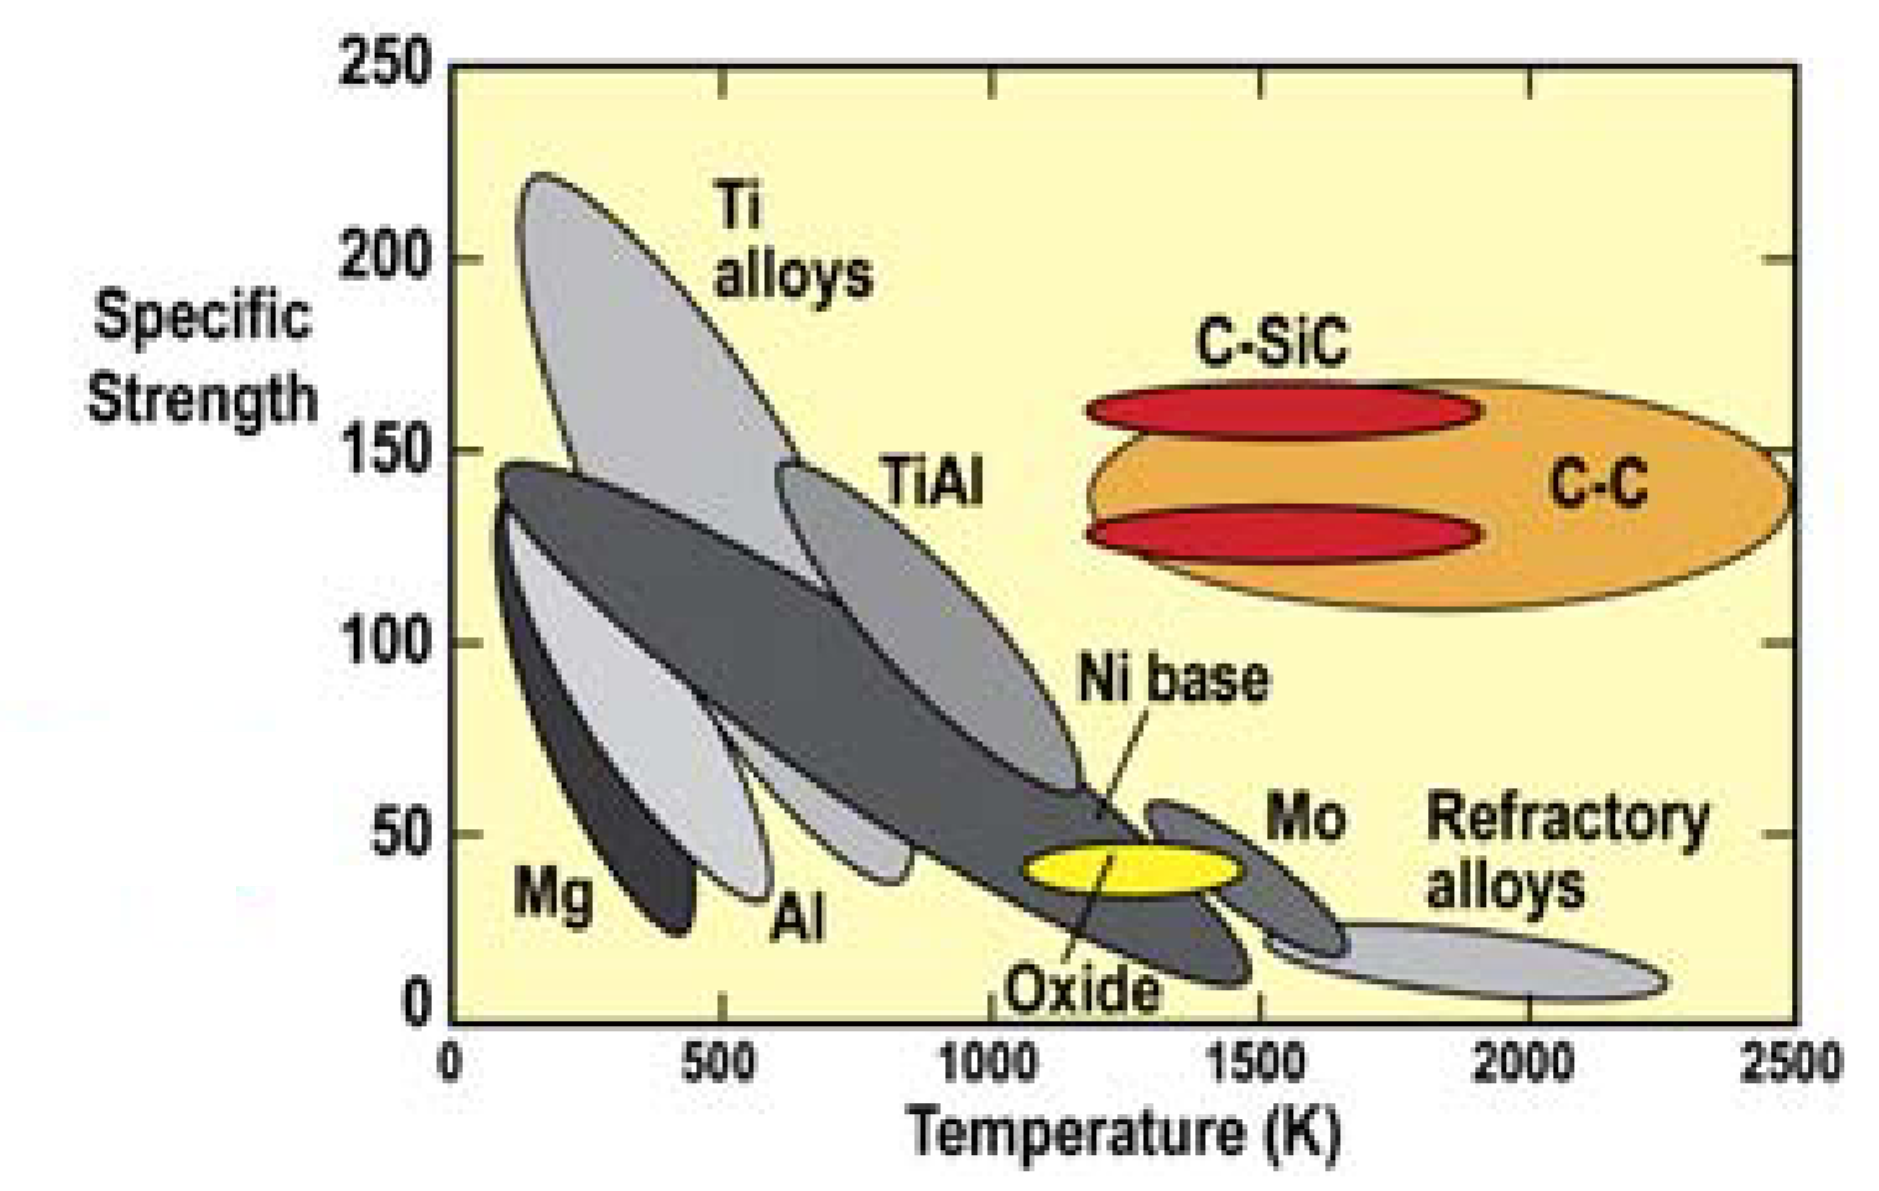
\includegraphics[width=\linewidth]{figures/Str_Temp.png}
        \caption{ }
    \end{subfigure}
    \hfill%
    \begin{subfigure}[t]{0.52\textwidth}
        \centering
        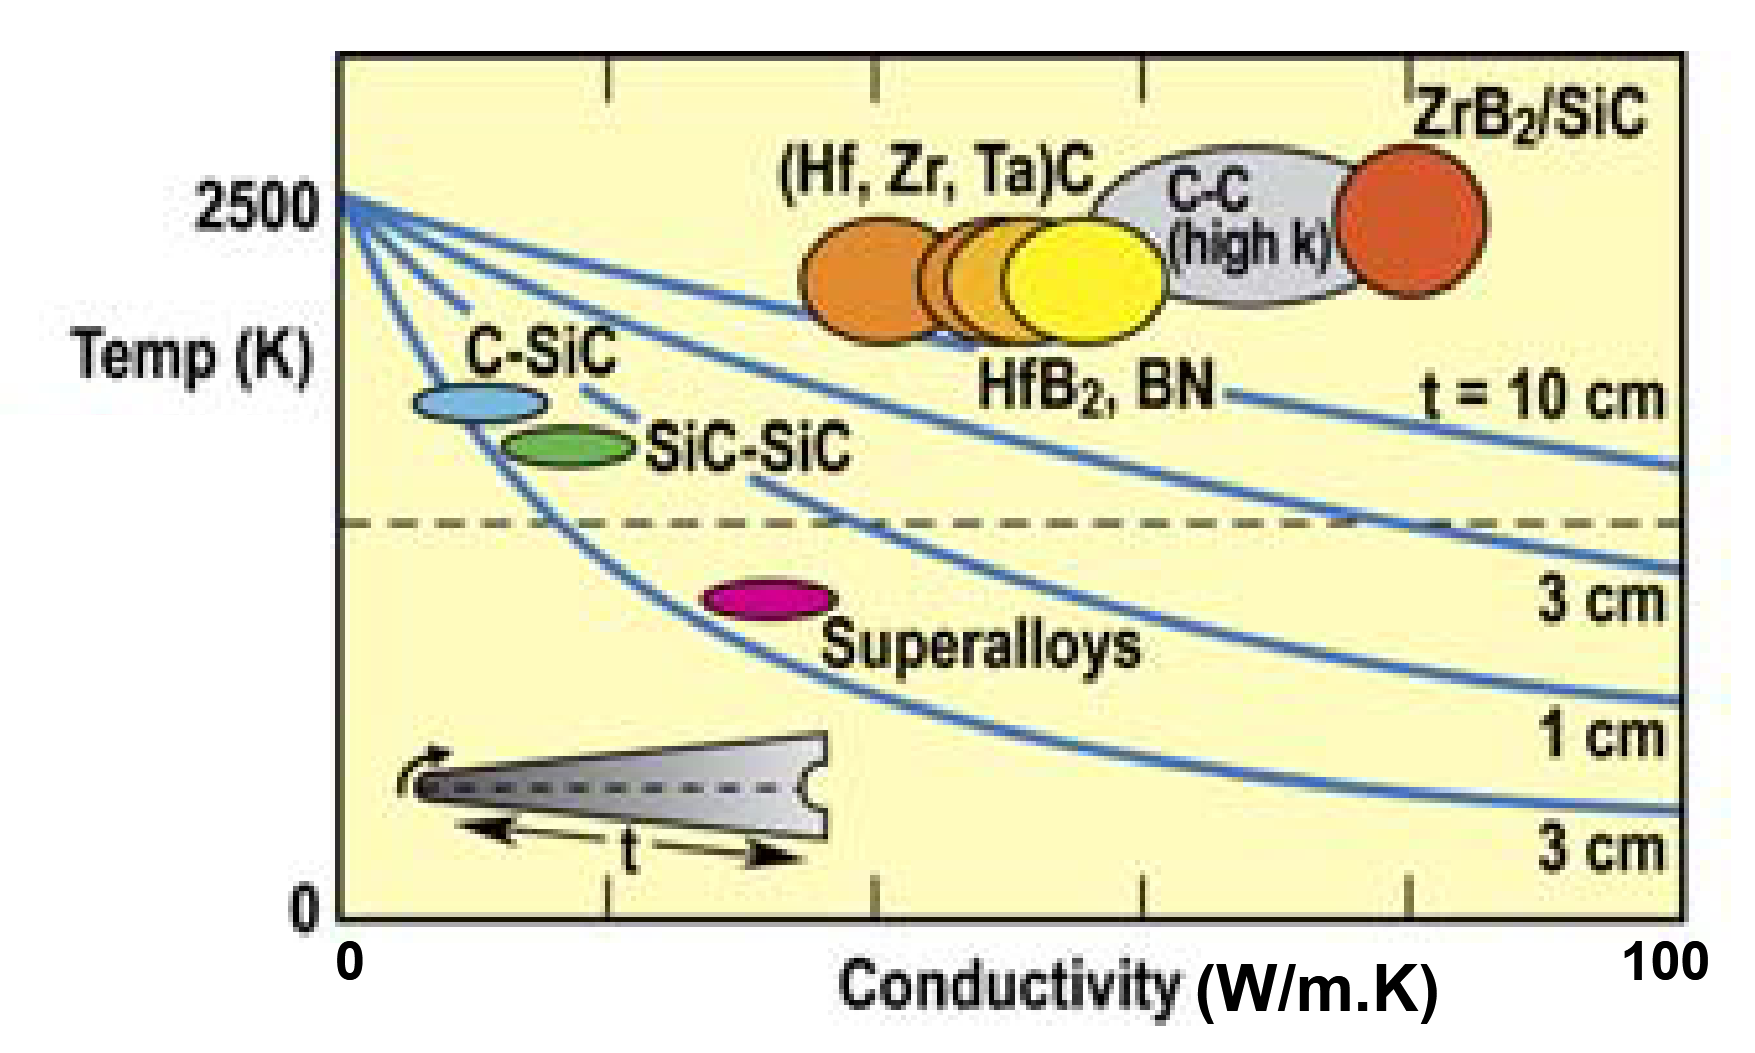
\includegraphics[width=\linewidth]{figures/Temp_Cond.png}
        \caption{}
    \end{subfigure}
    \caption{High-Temperature Aerospace Material Comparison \citep{DeStefanoFumo:2025}}
    \label{fig:materials}
\end{figure}

The selected material must not only maintain its structural integrity at $T_{\text{allow}}$, but also resist oxidation. High-performance metal alloys do not reach the required thermal limit. Refractory metals such as tungsten, with a melting point of 3695~K, suffer oxidation challenges at temperatures well below 2500~K. Recommended materials for hypersonic leading edges include refractory carbides/borides, such as Silicon carbide and Zirconium diboride, as well as C-C composites (\cite{DeStefanoFumo:2025}). C-C composites also suffer from oxidation at temperatures around 700 K, limiting their usefulness. CMCs seek to address the oxidation problem, and examples in use today use Silicon carbide or Silicon-infiltrated Silicon Carbide (SiSiC) as the matrix for a composite material (\cite{DeStefanoFumo:2025}). UHTCMCs are currently a theorized next step in high-temperature materials technology.

CMCs, specifically Carbon-fiber-reinforced Silicon Carbide, seem a reasonable leading edge material choice due to their high temperature limit, high conductivity, and high specific strength when heated. Furthermore, this material has been proven viable in high-temperature aerospace applications on the leading edges of the NASA Shuttle Orbiter, Sierra Space Dream Chaser, European Space Agency IXV, and the Soviet Buran spaceplane. 

\subsection{Powerplant selection}\label{sec:propulsion}
\subsubsection{Engine type}
The proposed vehicle uses a Scramjet engine to provide the thrust needed to maintain $M_\infty=6$ flight. Rocket engines, jet engines, and ramjet engines were considered but rejected for the present operating conditions:
\begin{itemize}
    \item Rocket engines were rejected because they fail to exploit the plentiful availability of atmospheric oxygen, instead requiring oxidizer to be carried. This increases the required propellant mass and results in low $I_{sp}$.
    \item Ramjets and jet engines were rejected because, at high Mach numbers, the freestream must be decelerated to subsonic speeds before combustion, as illustrated in\ \cref{fig:engines}, which produces large total-pressure losses and rapidly degrades efficiency.
\end{itemize}
At the chosen cruise condition ($M_\infty = 6$), scramjets become viable: by combusting fuel in a supersonic core flow, they avoid the large inlet total-pressure losses that hobble ramjets and turbojets at hypersonic speeds. Since takeoff and acceleration are outside the scope of this study, we assume the vehicle is already at its cruise operating point when the scramjets are engaged; in practice, a separate low-speed propulsion system or boost stage would be required to accelerate the vehicle through the subsonic and supersonic regimes up to the scramjet take-over Mach number.

\begin{figure}[htbp!]
    \centering%
    \begin{subfigure}[t]{0.45\textwidth}
        \centering
        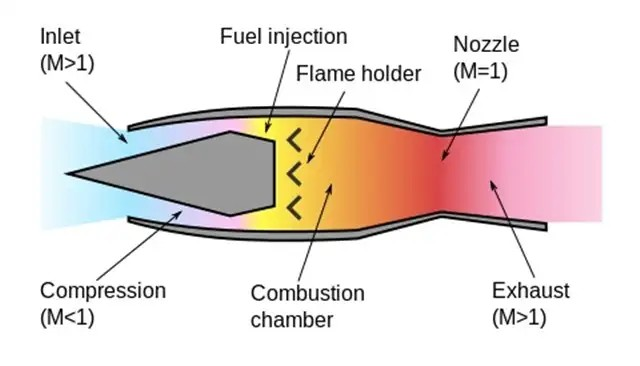
\includegraphics[width=\linewidth]{figures/Ramjet.jpg}
        \caption{Ramjet Engine}
    \end{subfigure}
    \hfill%
    \begin{subfigure}[t]{0.52\textwidth}
        \centering
        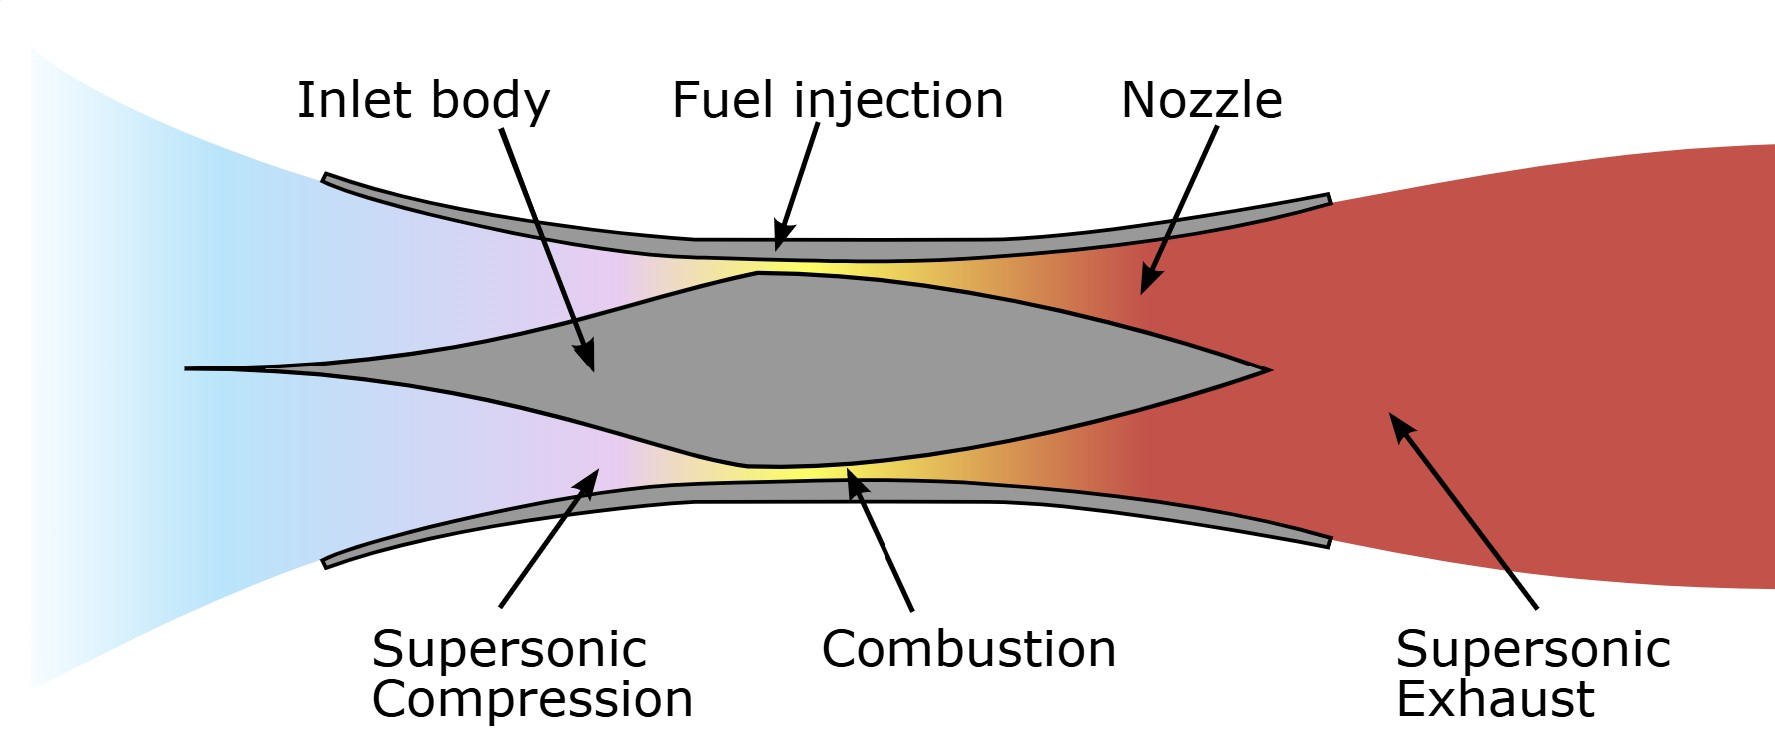
\includegraphics[width=\linewidth]{figures/Scramjet.jpg}
        \caption{Scramjet Engine}
    \end{subfigure}
    \caption{Comparison between Ramjet and Scramjet propulsion. Note the subsonic compression in the case of the Ramjet and the supersonic compression in the case of the Scramjet.\@ \citep{ramjetWiki}}
    \label{fig:engines}
\end{figure}

\subsubsection{Required thrust calculation}
The required thrust for the vehicle is estimated for steady, level Mach 6 cruise. Under this assumption, the vehicle is neither accelerating nor climbing, so the installed thrust requirement is set equal to the aerodynamic drag:
\begin{equation}
    T_{\mathrm{req}} = D = q_{\infty} S_{\mathrm{ref}} C_D,
\end{equation}
where \(q_{\infty}\) is the freestream dynamic pressure, \(S_{\mathrm{ref}}\) is the vehicle planform reference area, and \(C_D\) is the total drag coefficient. The dynamic pressure is calculated from the route-averaged atmospheric density and cruise velocity:
\begin{equation}
    q_{\infty} = \frac{1}{2} \rho_{\infty} V_{\infty}^2
    \quad\text{where}\quad
    V_{\infty} = M_{\infty} a_{\infty},\quad
    a_{\infty} = \sqrt{\gamma R T_{\infty}}
\end{equation}
where \(\gamma = 1.4\) is the ratio of specific heats for air, \(R = 287.05~\mathrm{J/(kg \cdot K)}\) is the specific gas constant for air, and \(T_{\infty}\) is the route-averaged freestream temperature. Substituting the aerodynamic characteristics of the optimal vehicle geometry from~\cref{sec:aerothermodynamics} gives:
\begin{equation}
    \boxed{T_{\mathrm{req}} = 204~\mathrm{kN}}
\end{equation}
This does not include additional thrust margin for acceleration, climb, maneuvering, inlet losses, installation losses, or off-design operation unless those effects are added separately.

\subsubsection{Engine Selection and Fuel Optimization Method}
\label{sec:range}
Following the definition of the vehicle, propulsion, and mission parameters, a discrete optimization routine was implemented to select the fuel type, engine count, and engine specific impulse that minimize takeoff mass. The optimizer is applied to the fixed waverider geometry, meaning the vehicle shape and internal volume are not modified during the trade study. Instead, the optimizer varies the propulsion and fuel parameters while holding the route, aerodynamic performance, vehicle volume, and cruise thrust requirement fixed.

The fuel requirement is calculated using the jet Breguet range relation,
\begin{gather}
    R = V I_{sp} g_0 \left(\frac{L}{D}\right) \ln\left(\frac{W_i}{W_f}\right),
\end{gather}
where \(R\) is the required range, \(V\) is the cruise velocity, \(I_{sp}\) is the engine specific impulse, \(g_0\) is standard gravity, \(L/D\) is the lift-to-drag ratio, and \(W_i/W_f\) is the initial-to-final weight ratio. Solving for the required weight ratio gives
\begin{gather}
    \frac{W_i}{W_f} = \exp\left[\frac{R}{V I_{sp} g_0 (L/D)}\right].
\end{gather}
The corresponding fuel mass is then
\begin{gather}
    m_f = m_{\mathrm{zf}}\left(\exp\left[\frac{R}{V I_{sp} g_0 (L/D)}\right]-1\right),
\end{gather}
where \(m_{\mathrm{zf}}\) is the zero-fuel mass of the aircraft, including the payload, airframe, and powerplant mass.

Fuel types considered are JP-7, liquid methane, and liquid hydrogen. The fuel properties and specific impulse ranges used in the optimizer are shown in Table~\ref{tab:fuel-options}. For each candidate fuel, the required fuel mass is converted into a storage volume according to its density. It must satisfy the constraint
\begin{gather}
    \frac{V_f}{V_{\mathrm{vehicle}}}\leq f_{\mathrm{fuel,max}},
\end{gather}
where \(V_{\mathrm{vehicle}}\) is the internal volume of the waverider and $f_{\mathrm{fuel,max}} = 15\%$ is the maximum allowable fuel volume fraction. Discrete numbers of engines from 2 to 16 were were considered, such that the available thrust exceeds the required cruise thrust with a 20\% margin. Each engine is limited to 60,000~N based on the reported performance of the strongest scramjet tested to date~\citep{Scram}. Thus, the minimum feasible engine count is six.

\begin{table}[htb]
\centering
\caption{Fuel properties and specific impulse ranges used in the Aircraft system optimizer.}
\label{tab:fuel-options}
\begin{tabular}{c|c|c|c}
\hline
\text{Fuel} &
\(\rho_f~[\mathrm{kg/m^3}]\) &
\(I_{sp,\min}~[\mathrm{s}]\) &
\(I_{sp,\max}~[\mathrm{s}]\) \\
\hline
\(\mathrm{JP\text{-}7}\) & 803.0 & 1000 & 2500 \\
\(\mathrm{Liquid\ methane}\) & 422.0 & 1000 & 2800 \\
\(\mathrm{Liquid\ hydrogen}\) & 70.8 & 1500 & 4000 \\
\hline
\end{tabular}
\end{table}

\begin{figure}[htb]
    \centering
    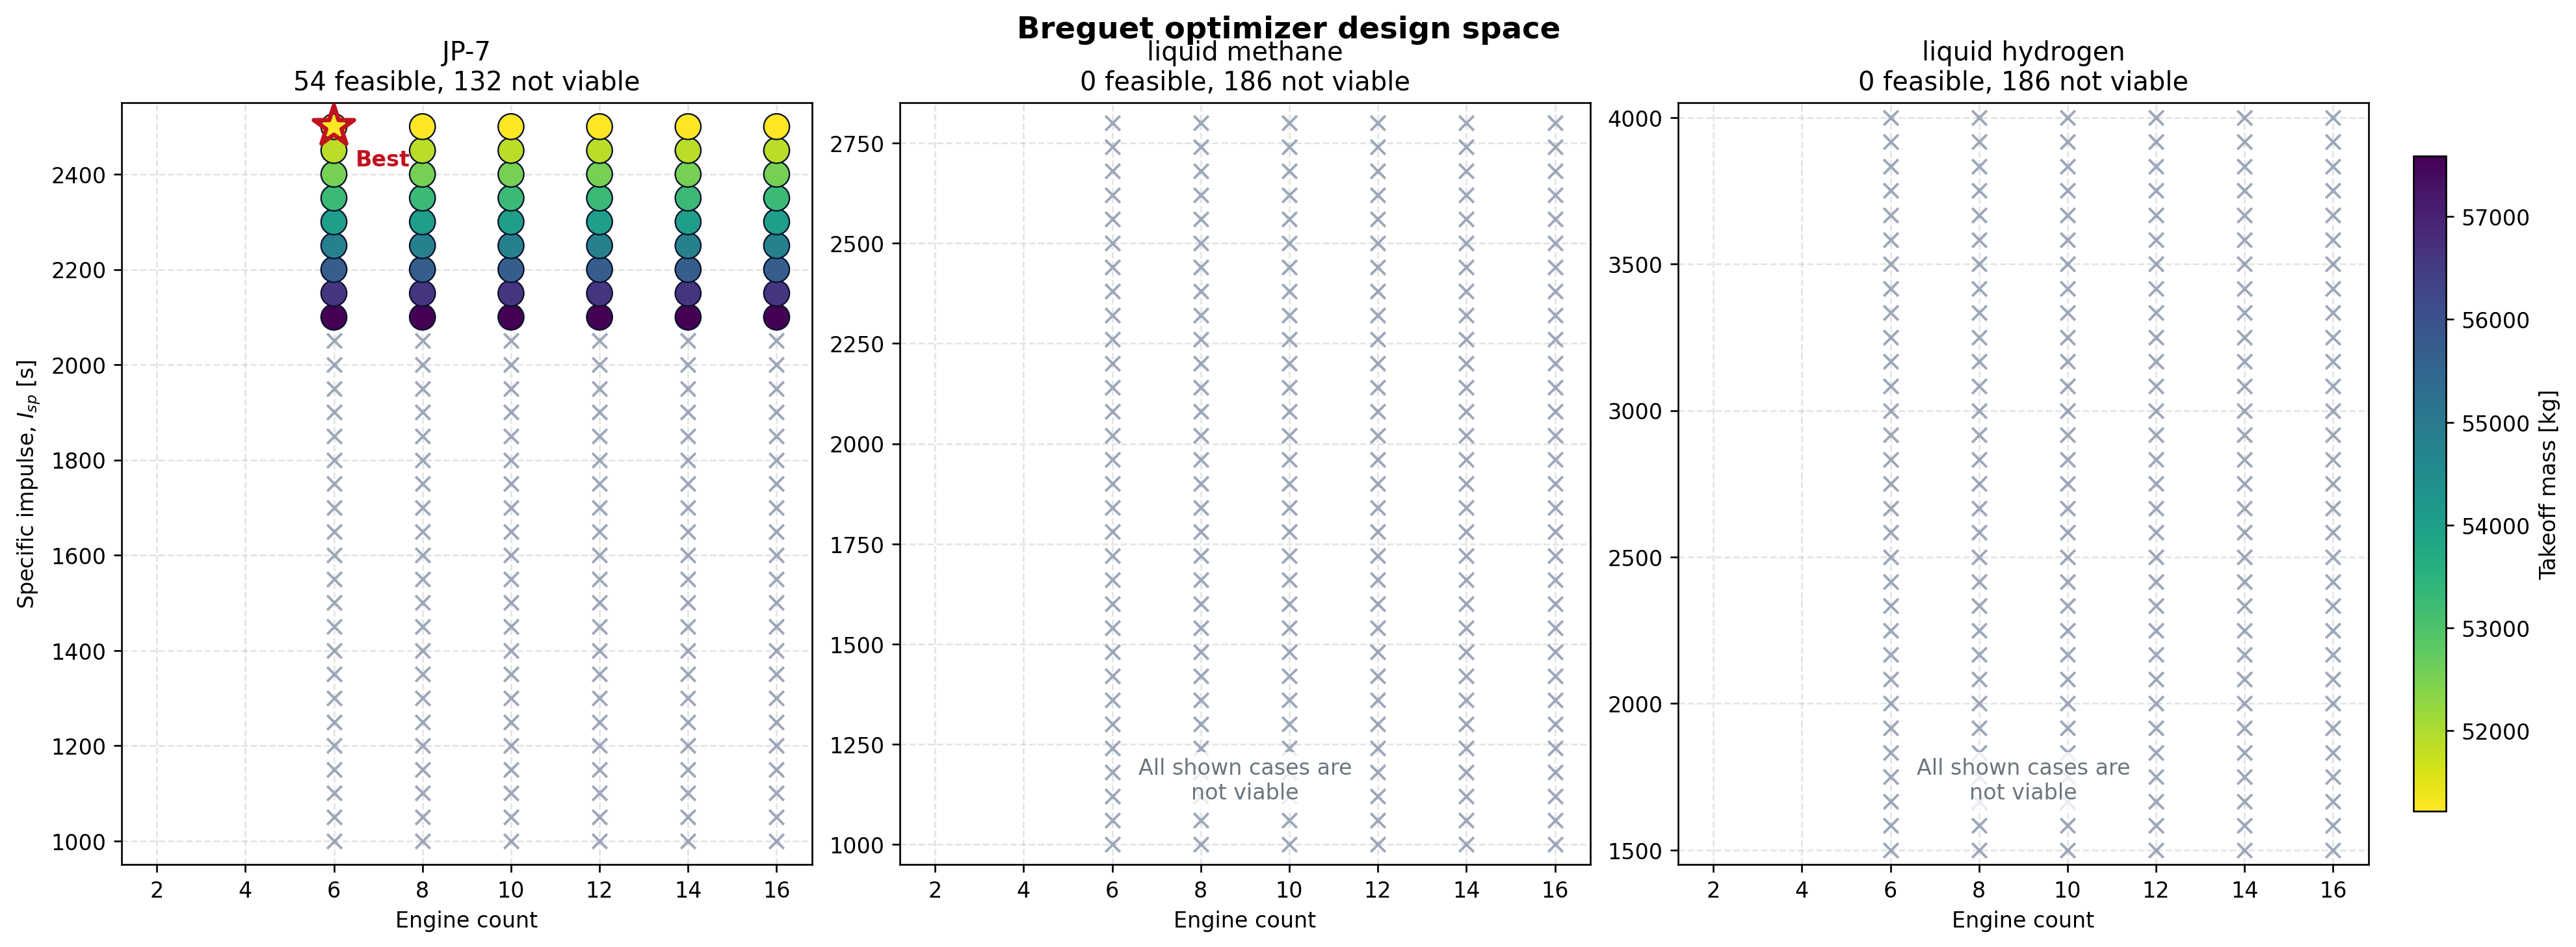
\includegraphics[width=1\linewidth]{figures/image.png}
    \caption{Viable Aircraft system optimizer cases by fuel option. Marker color denotes takeoff mass, and the red star marks the minimum-mass feasible case.}
    \label{fig:Breguet}
\end{figure}

\begin{table}[htb]
    \centering
    \caption{Unique viable Aircraft system optimizer options for the baseline configuration.}
    \begin{tabular}{lcccc}
        \hline
        Fuel & $I_{sp}$ [s] & Feasible engine counts & Fuel volume fraction & Takeoff mass [kg] \\
        \hline
        JP-7 & 2100 & 6, 8, 10, 12, 14, 16 & 14.90\% & 57,587.0 \\
        JP-7 & 2150 & 6, 8, 10, 12, 14, 16 & 14.41\% & 56,614.2 \\
        JP-7 & 2200 & 6, 8, 10, 12, 14, 16 & 13.96\% & 55,700.9 \\
        JP-7 & 2250 & 6, 8, 10, 12, 14, 16 & 13.53\% & 54,842.0 \\
        JP-7 & 2300 & 6, 8, 10, 12, 14, 16 & 13.13\% & 54,032.8 \\
        JP-7 & 2350 & 6, 8, 10, 12, 14, 16 & 12.75\% & 53,269.3 \\
        JP-7 & 2400 & 6, 8, 10, 12, 14, 16 & 12.39\% & 52,547.7 \\
        JP-7 & 2450 & 6, 8, 10, 12, 14, 16 & 12.05\% & 51,864.7 \\
        JP-7 & 2500 & 6, 8, 10, 12, 14, 16 & 11.73\% & 51,217.4 \\
        \hline
    \end{tabular}
    \label{tab:breguet-optimizer-viable-options}
\end{table}


A sweep 744 of fuel type, engine count, and specific impulse combinations were swept for the optimized geometry from~\cref{sec:aerothermodynamics}. Only cases satisfying both the fuel-volume constraint and the thrust-availability constraint are considered feasible. Of these, 54 cases (7.3\%) were feasible. The minimum-mass feasible case used JP-7 with $I_{sp}=2500\,\mathrm{s}$ and 6 engines. This case required $29.3\,\mathrm{m}^{3}$ of fuel (11.73\% of vehicle volume) and produced a takeoff mass of $51,217.4\,\mathrm{kg}$. Within the feasible design space, increasing specific impulse monotonically reduced both fuel-volume fraction and takeoff mass. This indicates that propulsion efficiency, rather than additional engine multiplicity, is the dominant lever in the present aircraft systems optimizer. The non-viable fuels were screened out by the fuel-volume constraint rather than the thrust constraint. With the current thrust requirement, engine counts of 6 to 16 all satisfy requirements. For liquid methane, even the best thrust-feasible case (6 engines and $I_{sp}=2800\,\mathrm{s}$) required $20,269.9\,\mathrm{kg}$ of fuel, which corresponds to $48.0\,\mathrm{m}^{3}$ or 19.21\% of vehicle volume. For liquid hydrogen, even the best thrust-feasible case (6 engines and $I_{sp}=4000\,\mathrm{s}$) required $12,983.2\,\mathrm{kg}$ of fuel, which corresponds to $183.4\,\mathrm{m}^{3}$ or 73.35\% of vehicle volume. This comparison shows that the present trade study is volume-limited for cryogenic fuels: higher specific impulse reduces fuel mass, but the lower fuel density overwhelms that benefit once the storage-volume cap is enforced.

\subsection{Final summary of systems}
Below is a summary table of the aircraft systems, as determined by the system optimization scheme.

\begin{table}[htbp]
    \centering
    \caption{Final aircraft system summary.}
    \label{tab:breguet-final-system-summary}
    \begin{tabular}{lr}
        \hline
        System / Category & Value \\
        \hline
        Mission range & $15{,}900~\mathrm{km}$ \\
        Cruise altitude & $70{,}000~\mathrm{ft}$ \\
        Cruise Mach number & $6.0$ \\
        Mean cruise speed & $1{,}776~\mathrm{m/s}$  \\
        Time of flight & $2.5~\mathrm{hr}$  \\
        Vehicle volume & $250~\mathrm{m^3}$ \\
        Lift-to-drag ratio & $5.82$ \\
        Required thrust & $203{,}700~\mathrm{N}$ \\
        Max thrust per engine & $60{,}000~\mathrm{N}$ \\
        Selected fuel & JP-7 \\
        Fuel density & $803.0~\mathrm{kg/m^3}$ \\
        Specific impulse & $2{,}500~\mathrm{s}$ \\
        Engine count & $6$ \\
        Total powerplant mass & $2{,}500~\mathrm{kg}$  \\
        Required fuel mass & $23{,}500~\mathrm{kg}$ \\
        Required fuel volume & $30~\mathrm{m^3}$ \\
        Fuel volume fraction & $12\%$ \\
        Payload mass & $9{,}820~\mathrm{kg}$ \\
        Airframe mass & $15{,}360~\mathrm{kg}$ \\
        Zero-fuel mass & $27{,}680~\mathrm{kg}$ \\
        Takeoff weight & $502~\mathrm{kN}$ \\
        Selected Leading Edge Material & C-Reinforced SiC \\
        Payload mass fraction & $20\%$ \\
        Powerplant mass fraction & $5\%$ \\
        Fuel mass fraction & $46\%$ \\
        \hline
    \end{tabular}
\end{table}

% ==========================================================================
% \FloatBarrier%
\section{Limitations \& future work}

``It is really not foreseeable that an `optimized' calculated shape could do anything more than give a guide to the designer.\@ [\ldots\ The designer] would really be a little embarrassed to be offered a perfect aerodynamic shape, which he would then have to carve holes in, add fairings, and so on, in order to satisfy such mundane requirements as that the pilot should be able to see where he is going or that people have somewhere convenient to get in and out.'' --- Phillip Roe, 1970

The present preliminary design rests on several modeling simplifications, each of which introduces a clear avenue for refinement. Foremost among these, the aerodynamic analysis assumes steady, laminar, attached, continuum flow with a calorically perfect gas. At Mach~6 and 70{,}000~ft, real-gas effects (vibrational excitation and incipient dissociation) and laminar---turbulent transition along the lower surface are both plausible, and either would alter the predicted drag and heating; incorporating a high-temperature equation of state and a transition criterion would tighten these estimates. Base drag is neglected because separation is not modeled, and viscous-inviscid interaction and shock--boundary-layer interaction are likewise omitted; while we have argued that these are small in the design regime, they should be revisited in a higher-fidelity CFD campaign. The blunt leading edge is treated with a uniform stagnation-point heating estimate (Sutton--Graves) and a Newtonian pressure correction, rather than a spanwise-resolved aerothermal calculation that would allow a tapered leading-edge radius and yield a less conservative wave-drag penalty.

On the systems side, the airframe mass is scaled from a Boeing~737 reference density and does not reflect the thermal-protection mass premium or the structural penalty of carrying cryogenic tanks. The propulsion model assumes a constant engine thrust-to-weight ratio of 8.3, an idealized fixed per-engine thrust limit, and a fixed specific impulse over the cruise; it does not capture inlet--engine--airframe integration, off-design performance, or the takeoff/acceleration phase needed to reach the scramjet operating envelope. Finally, geometric features required by any real passenger vehicle---windows, doors, control surfaces, landing gear, engine nacelles, and stability augmentation surfaces---are absent from the optimized waverider and would each modify the aerodynamic performance reported here. Future work should therefore proceed by coupling the present analysis with (i) a turbulent, real-gas CFD evaluation of the optimized geometry, (ii) a sized thermal-protection and structural mass model, and (iii) an integrated propulsion model spanning the full acceleration and cruise profile.

\section{Software availability}
The methods described in this report were implemented in the Python programming language. The complete software is available in the GitHub repository {\small\url{https://github.com/trulko/hypersonic-waverider}}.


% ==========================================================================
\FloatBarrier%
\printbibliography%

\end{document}
